% TeXplates/Mathematics.tex
% v0.2.1
% https://github.com/HoyanMok/TeXplates
\documentclass[openany, a5paper, oneside]{ctexbook} 
% \documentclass{ctexbook} 如果用中文
% \documentclass[10pt,a4paper]{ctexart}  字体大小和纸张大小,默认分别为10pt和letterpaper
% 五号 = 10.5pt,小四=12pt,四号=14pt
% 其他可选参量如twocolumn, 两行排版

\usepackage{../TeXplatesMathematics}

\addbibresource{Algebra.bib} % 把这里改成实际的文件名


\newcommand*{\inbasis}[2]{\left.%
	{#1}\right|_{#2}
}

\DeclareMathOperator{\rank}{rank}
\DeclareMathOperator{\lcm}{lcm}
\DeclareMathOperator{\pp}{pp}

\DeclareMathOperator{\characteristic}{char}
\DeclareMathOperator{\codim}{codim}
\DeclareMathOperator{\End}{End}
\DeclareMathOperator{\tr}{tr}
\DeclareMathOperator{\Spec}{Spec}


\newcommand*{\Orth}{\mathrm{O}}
\newcommand*{\GF}{\mathrm{GF}}
\newcommand*{\Cl}{\mathrm{Cl}}




% 文章标题页信息:
\title{Algebra}
\author{ Hoyan Mok\thanks{E-mail: victoriesmo@hotmail.com}
	}
\date{\today} % 自动生成日期
\titlepic{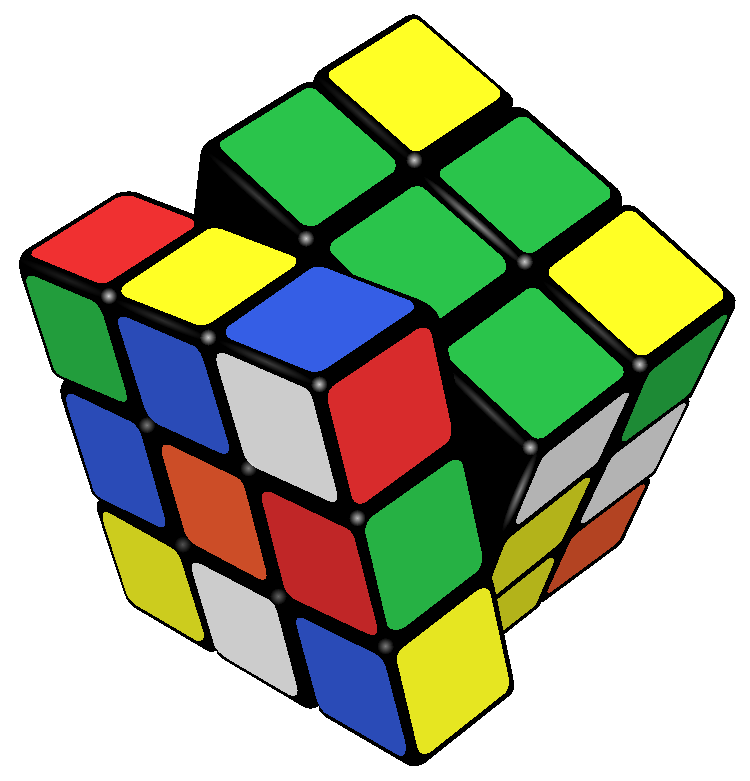
\includegraphics[width=8 cm]{Rubik's_cube.pdf}}

\begin{document}
\pagenumbering{Alph}
\maketitle % 打印标题
\thispagestyle{empty}
\frontmatter
\chapter{笔记说明}
本笔记是笔者学习线性代数时做的, 主要参考资料是\cite{代数学引论第二卷}. 

笔记假定读者已经熟悉朴素集合论的术语与符号, 并已经学习了以矩阵和行列式运算为主的初级线性代数. 
但本笔记力求自足, 将矩阵与行列式运算, 置换和多项式等内容附在附录中, 以资读者在阅读正文时可以随时查阅.

笔记后附有符号列表和索引, 方便读者 (也是方便笔者自己) 查阅.

你可以在 \url{https://github.com/HoyanMok/NotesOnMathematics/tree/master/Algebra} 获得本笔记最新的PDF与\TeX{}源文档. 
封面的来源是 \url{https://commons.wikimedia.org/wiki/File:Rubik%27s_cube.svg}.

\tableofcontents

\mainmatter{}
\part{线性代数}
\chapter{群. 环. 域}
\section{代数运算}
\begin{definition}[二元运算]
	集合的Cartesian平方到自身的映射$* \colon X^2 \to X$称为其上的一个\indexbf{二元运算}.
	通常我们记$*(a,b) := a * b$. 
	当$X$上定义了二元运算$*$后, 称$*$定义了$X$上的一种\indexbf{代数结构} $\indexmath[X ast]{(X,*)}$, 也称\indexbf{代数系统}. 
\end{definition}

当指代是明确的时候, 我们将混用集合及其代数结构.

作为习惯, 如果$\cdot, + \in X^{X^2}$, 我们记$ab := a \cdot b$并称其为$a$和$b$的\indexbf{积}, 称$a+b$为$a$和$b$的\indexbf{和}. 这些只是约定.

若$a* b = b* a$则称$*$或$(X,*)$是\indexbf{交换的}, 而若$(a* b)* c = a*(b* c)$则称$*$或$(X,*)$为\indexbf{结合的}. 

若$\exists e\in X$满足$\forall x\in A\big(
	e* x = x * e = x
\big)$, 则称其为$*$的一个\indexbf{单位元} (identity), 这时可把$(X,*)$记作$\indexmath[X ast e]{(X,*, e)}$. 可以证明一个代数结构最多只有一个单位元. 
乘法单位元通常记为$1$, 而加法单位元 (也叫\indexbf{零元}) 记为$0$.

\begin{definition}[半群和幺半群]
	若$*$是结合的, 称$(X,*)$是\indexbf{半群} (semigroup); 
	若$*$还有一个单位元, 则称$(X,*, e)$是\indexbf{幺半群} (monoid).
\end{definition}

倘若幺半群$(M, *, e)$是有限的 (即其元素有限), 称$\card M$为\indexbf{有限幺半群}的\indexbf{阶}.

作为重要的例子, \indexbf{置换幺半群} 定义为$(X^X, \circ, \id_X)$, 有幺半群结构的$X^X$通常记作$M(X)$.

半群中, 括号的位置是不重要的 (可用数学归纳法证明). 通常我们记$x_1x_2 \cdots x_n$为:
\begin{equation}
	\prod_{i=1}^1 x_i = x_1,\;\prod_{i=1}^{n+1} x_i = \left( \prod_{i=1}^n x_i  \right) x_n\,;
\end{equation}
同理$x_1+x_2+\cdots + x_n$为:
\begin{equation}
	\sum_{i=1}^1 x_i = x_1,\;\sum_{i=1}^{n+1} x_i = \left( \sum_{i=1}^n x_i  \right) + x_n\,.
\end{equation}
在半群不交换的场合, 指出递推式右端的顺序是重要的. 这种记法称为\indexbf{左正规}.

若$x := x_1 = x_2 = \cdots = x_n$, 记$\sum_{i=1}^n x_i = nx$, $\prod_{i=1}^n x_i = x^n$, 分别表示$x$的$n$倍和$x$的$n$次幂. 它们满足:
\begin{equation}
	nx+mx = (n+m)x, \; n(m x) = nm x, \qquad n,m\in \mathbb N_+\,;
\end{equation}
\begin{equation}\label{exoponentiation}
	x^n x^m = x^{n+m}, \; (x^m)^n = x^{nm}, \qquad n,m \in \mathbb N_+\,.
\end{equation}

在幺半群中, 还可以令$x^0 = 1$, $0x = 0$.

若半群$S$有子集$S'$, 使得$(S',*)$是半群, 那么称其为半群$(S,*)$的\indexbf{子半群}.
同理有幺半群\nolinebreak$M$的\indexbf{子幺半群}$M'$. 

若半群$(S,*, e)$的元素$a$满足$\exists a'\in S\big(
	a a' = a' a = e
\big)$, 那么称$a$为\indexbf{可逆的} (invertible), $a'$称为其\indexbf{逆元} (inverse element) 或\indexbf{逆} (inverse).
通常加法逆元记为$- a$, 乘法逆元记为$a^{-1}$, 且为可逆元素引入$n a$, $a^n$的概念, 其中$n \in \mathbb Z$. 当$n$为负数时, $na = -(-na)$, $a^n = (a^{-n})^{-1}$.

因为群未必是Abelian, 我们可以也用弱化的\indexbf{左可逆} $\exists y$ s.t.\ $y * x = 1$或\indexbf{右可逆}的概念.


\section{群}\label{section:群}
可逆幺半群$G$称为群, 即:
\begin{definition}[群]
	设有集合$G$. 若:
	\begin{conditionlist}[label=G\arabic*)]\setcounter{enumi}{-1} % chktex 9
		\item 定义了二元运算$\mathord{\cdot} \colon G^2 \to G; (x,y) \mapsto xy$.
		\item 结合性: $\forall x,y,z\in G$, $(xy)z = x(yz)$.
		\item 单位元: $\exists e\in G \forall x\in G$, $xe = ex = x$.
		\item 可逆性: $\forall x\in G \exists x^{-1} \in G$, $x x^{-1} = x^{-1} x = e$.
	\end{conditionlist}
	则称$(G, \cdot)$为\indexbf{群}.
\end{definition}

交换群又叫做\indexbf{Abelian群}. 

作为重要的例子, 设 $X$ 是一个集合, $\indexmath[S X]{S(X)} = \{ f \in X^X \mid \text{$f$ 是双射}\}$. 
我们断言, $(S(X), \circ, \id_X)$ 是一个群, 称为\indexbf{变换群}或\indexbf{置换群}, 其中 $\circ$ 是函数的复合, $\id_X$是恒等变换. 
当它的阶数 $\card X = n$ 是有限的时候, 记$\indexmath[S n]{S_n} := S(X)$.

群也有子群的概念. 
设$(G, \cdot, e)$是一个群. 当一个集合$G' \subset G$满足:
\begin{conditionlist}[label=SG\arabic*)]
	\item $e \in G'$;
	\item $\forall x,y\in G'$, $xy \in G'$;
	\item $x \in G' \to x^{-1} \in G'$,
\end{conditionlist}
则称$(G', \cdot , e)$是一个$G$的\indexbf{子群}.
倘若还有$G' \neq G$则称其为一个\indexbf{真子群}\footnote{\cite{kostrikin1982introduction}等文献把\indexbf{平凡群} $\{e\}$ 也排在真子群的定义外.}.

\begin{theorem}
	非空的 $G'$ 是群 $(G, \cdot, 1)$ 的子群 $\IFF$ $\forall x,y \in G' (xy^{-1} \in G')$.
\end{theorem}
\begin{proof} 
	根据子群的定义, $\to$ 是显然的, 下给出 $\gets$ 的证明:
	\begin{conditionlist}[label=SG\arabic*)]
		\item $\forall x \in G' (x x^{-1} = 1 \in G)$;
		\item $\forall x,y\in G'$, $x1^{-1} (1y^{-1})^{-1} = xy \in G'$;
		\item $\forall x \in G'$, $1x^{-1} = x^{-1} \in G'$.
	\end{conditionlist}
\end{proof}

这里将不加证明地给出:
\begin{lemma}\label{theorem: 子群族的交}
	群 $G$ 的子群族 $\mathscr H = \{H \mid \text{$H$ 是 $G$ 的子群}\}$ 的交 $\cap \mathscr H$ 也是 $G$ 的子群.
\end{lemma}

设 $G$ 有子集 $S$, 我们说群 $(G, \cdot, 1)$ 是由 $S$ 生成的, 意思是说 $G$ 没有包含 $S$ 的真子群. 记为$G = \indexmath[S]{%
	\langle S\rangle}$.
\begin{theorem}
	$\langle S \rangle = \left\{
		\prod^{n-1}_{i=0} s_i \middle|
			\forall i \in n(s_i \in S \vee s_i^{-1} \in S)
\right\}$.
\end{theorem}
\begin{proof}
	根据群的定义, 形如 $\prod^{n-1}_{i=0} s_i$ 的将构成一个群. 如果存在一个不能写成这种形式的元素, 那么它们将构成一个真子群, 这和 $\langle S\rangle$的定义相违背. 
	
\end{proof}

我们把半群的公式~\eqref{exoponentiation} 推广到整数次幂, 证明在此忽略了.
\begin{theorem}\label{group exoponentiation}
	$\forall g \in G$, $\forall n,m\in \mathbb Z$,
	\begin{equation}
		g^m g^n = g^{m+n}, \quad
		(g^m)^n = g^{mn}.
	\end{equation}
\end{theorem}

\begin{definition}[循环群]
	设$(G, \cdot , 1)$是一个乘法群, $\exists g_0 \in G$, 使得$\forall g \in G$, $\exists n \in \mathbb Z$, $a^n = g$, 那么我们称它是一个\indexbf{循环群}, $g_0$是一个\indexbf{生成元} (generator), 并记作$G = \indexmath[g 0]{\langle g_0 \rangle}$.
\end{definition}

对于群 $G$ 中任意元素 $g$, 我们称 $\card \langle g \rangle$ 为元 $g$ 的\indexbf{阶数}, 或称 $g$ 为 \emphbf{$n$~阶元}%
	\index{n阶元@$n$~阶元}. 
	而且它将满足:
\begin{theorem}
	任意群 $G$ 中若有 $q \in \mathbb Z$ 阶元 $g$, 则 $\langle g \rangle = \{e, g, \dots, g^{q-1}\}$, 且:
	\begin{equation}
		g^n = e \IFF n = kq, \qquad n \in \mathbb Z\,.
	\end{equation}
\end{theorem}
证明利用带余除法和定理~\ref{group exoponentiation}, 证明是显然的. 从该定理, 我们可以论断: 循环群都是Abelian群.

\begin{definition}[同构]
	两个群 $(G, *)$, $(G', \circ)$ 如若满足: $\exists f\colon G \to G'$ s.t.\ \begin{conditionlist}[label=\roman*)]
		\item $\forall a, b \in G$, $f(a * b) = f(a) \circ f(b)$; \label{item: 保结构}
		\item $f$是双射,
	\end{conditionlist}
	则称 $f$ 是一个\indexbf{同构映射}或\indexbf{同构} (isomorphism), 并认为两个群是互相\indexbf{同构}的 (isomorphic), 记为$\indexmath[G simeq G prime]{G \simeq G'}$.
\end{definition}

同构关系的自反性, 传递性和对称性是平凡的.

\begin{theorem}
	设群 $(G, *, 1)$, $(G', \circ, 1')$ 被 $f$ 见证同构, 那么$f(1) = 1'$.
\end{theorem}
\begin{proof}
	$\forall g' \in G'$, 记 $g := f^{-1}(g')$, 那么 $f(g)\circ f(1) = f(g * 1) = g' = f(1 * g) = f(1) \circ f(g)$. 从而$f(1) = 1'$.
\end{proof}

\begin{theorem}
	设群 $(G, *, 1)$, $(G', \circ, 1')$ 被 $f$ 见证同构, 那么$\forall g \in G$, $f(g^{-1}) = f(g)^{-1}$.
\end{theorem}
\begin{proof}
	$f(g) \circ f(g^{-1}) = f(g * g^{-1}) = f(1) = 1' 
		= f(g^{-1} * g) = f(g^{-1})\circ f(g)$.
\end{proof}

\begin{theorem}
	\begin{equation*}
	\card \langle g_0\rangle = \card \langle g'_0 \rangle 
		\to \langle g_0\rangle \simeq \langle g'_0 \rangle\,.
	\end{equation*}
\end{theorem}
\begin{proof}
	倘若$\card \langle g_0\rangle = \infty$, 那么$\nexists n \in \mathbb Z - \{0\}$, s.t.\ $g_0^n = e$; 这意味着, 存在这样的双射 $f\colon \mathbb Z \to \langle g_0\rangle$, 满足$f(n) = g_0^n$, 见证了 $(\mathbb Z, +, 0) \simeq (\langle g_0\rangle , *, e)$. 

	如果阶数是有限的, 只需令$f\colon g^k \to g'^k$, 其中$k= 0$, $1$, $\cdots$, $\card\langle g_0\rangle$.
\end{proof}

\begin{theorem}[\indexbf{Cayley定理}]
	设 $(G, *, e)$ 任意 $n$ 阶有限群. 
	$\exists H \subset S_n$ s.t.\ $(H, \circ,\id_X)$是$S_n$的子群且 $G \simeq H$. 
\end{theorem}
\begin{proof}
	取$H := \{L_g \mid g \in G\}$, 其中$L_g \colon G \to G; g' \mapsto gg'$可以证明是双射. 那么 $L\colon G \to H; g \mapsto L_g$ 见证了 $H \simeq G$.
\end{proof}

若 $\varphi \colon G \to G$ 见证了 $G \simeq G$ (如 $\id_G$), 那么称 $\varphi$ 是群 $G$ 的一个 \indexbf{自同构} (automorphism). 所有自同构组成的集合 $\indexmath[Aut G]{\Aut(G)}$ 和其上的函数复合 $\circ$ 构成了 $S(G)$ 的一个子群, 称为$G$的\indexbf{自同构群}.

自同构群有一特殊的子群$\indexmath[Inn G]{\Inn(G)} := \{I_a \colon g \mapsto a g a^{-1} \mid a \in G\}$,
称为\indexbf{内自同构群} (inner isomorphism), 其元素称为\indexbf{共轭映射} (conjugation). 

\begin{definition}[共轭]
	设 $G$ 是一个群, $a, b \in G$. 如果 $\exists I_g \in \Inn(G)$, 使得 $I_g(a) = b$, 那么我们称 $a$ 和 $b$ 互为\indexbf{共轭} (conjugate).
\end{definition}

我们毫不费力地就能证明共轭关系是等价关系, 而且当 $G$ 是Abelian群的时候, 其任意元素的共轭都是其自身.

\begin{definition}[共轭类]
	设 $G$ 是一个群. 由共轭规定的等价类称为\indexbf{共轭类} (Conjugacy class), 记为 $\indexmath[Cl g]{\Cl(g)}$, $g$ 为其代表元. 
	称 $\card \{ \Cl(g) \mid g \in G\}$ 为 $G$ 的\indexbf{类数} (class number). 
	如果有一个函数 $f$ 满足 $g' \in \Cl(g) \,\to\, f(g) = g(g')$, 那么称 $f$ 是一个 \indexbf{类函数} (class function).
\end{definition}

\begin{definition}[正规子群]
	设 $G$ 是一个群, $N$ 是其子群. 倘若 $\forall I \in \Inn(G)$, $I(N) = N$, 即其在共轭映射下不变, 则称其为 $G$ 的一个\indexbf{正规子群} (normal subgroup), 记为 $\indexmath[N triangleleft G]{N \triangleleft G}$.
\end{definition}

可以看出Abelian群的所有子群都是正规子群. 
以下是正规子群的另一种定义方法:
\begin{theorem}
\begin{equation*}
	N \triangleleft G \IFF
		\forall g, h \in G\; (gh \in N \IFF hg \in N)\,.	
\end{equation*}
\end{theorem}
\begin{proof}
	只需注意到 $I_g(gh) = g^{-1} gh g = hg$.
\end{proof}


\begin{definition}[同态]
	设有群 $(G, *, e)$ 和 $(G', \circ, e')$, 映射 $f \colon G \to G'$ 若满足
	\begin{equation*}
		\forall a, b \in G, \quad 
			f(a * b) = f(a) \circ f(b),
	\end{equation*}
	则称其为群 $(G, *)$ 到群 $(G', \circ)$ 的一个\indexbf{同态} (homomorphism), 也叫\indexbf{态射} (morphism). 类似映射, 可定义\indexbf{单态射} (monomorphism), \indexbf{满态射} (epimorphism).

	集合 $\indexmath[ker f]{\ker f} := f^{-1}(\{e'\})$ 叫做同态 $f$ 的\indexbf{核} (kernel). 群到自身的同态映射称为\indexbf{自同态} (endomorphism).
\end{definition}

同态 $f$ 的核是 $G$ 的正规子群, 即$\ker f \triangleleft G$, 而 $G$ 在同态下的像是 $G'$ 的子群.

\begin{theorem}
	如果同态的核是平凡群(即, $\ker f = \{e\}$), 那么这个同态是单的.
\end{theorem}
\begin{proof}
	如果$\exists g_1, g_2 \in G$, s.t.\ $f(g_1) = f(g_2)$, 
	那么
	\begin{align*}
		f(g_1 * g_2^{-1}) 
		&= f(g_1) \circ f(g_2^{-1}) 
		= f(g_1) \circ f(g_2)^{-1} \circ f(g_2) \circ f(g_2^{-1})
		//
		&= e' \circ f(e)
		= e'
	\end{align*}
	从而$g_1 * g_2^{-1} \in \ker f$, 同理$g_2^{-1} * g_1 \in \ker f$, 即$g_1^{-1} = g_2^{-1}$ 或 $g_1 = g_2$, 即: $f$是单的.
\end{proof}

作为例子, 映射
\begin{equation*}
	f \colon G \to \Inn(G);\, g \mapsto I_g
\end{equation*}
满足同构的条件~\ref{item: 保结构}, 因$f(a) \circ f(b) = I_{ab} = f(ab)$; 但它不一定是双射, 因而是一个同态.

\begin{definition}[陪集]
	设 $(G, *, e)$ 是一个群, $S$ 是其子群, $g \in G$, 那么我们称 $\indexmath[g ast S]{g * S} := \{ g * s \mid s \in S\}$ 为 $S$ 在 $G$ 内的\indexbf{左陪集} (left coset); 
	同理 $\indexmath[S ast g]{S * g} := \{ s * g \mid s \in S\}$ 为 $S$ 在 $G$ 内的\indexbf{右陪集} (right coset). 
	这里我们称 $g$ 是一个代表元.
	如果 $g * S = S * g$, 则称其为\indexbf{陪集}.
\end{definition}

\begin{theorem}
	\begin{equation*}
		N \triangleleft G 
			\IFF \forall g \in G,\; g * N = N * g.
	\end{equation*}
\end{theorem}

\begin{definition}[商群]
	如果 $N \triangleleft G$, 那么我们记 $\indexmath[G N]{G / N} := \{ g * N \mid g \in G\}$, 称为 $G$ 对 $N$ 的\indexbf{商群}. 
	这个群的乘法定义为子群元素的积的集合: 
	\begin{equation*}
		(g * N) \cdot (g'* N)
		:= \{s * t \mid s \in g * N, \; t \in g; * N\} 
		= (g * g') * N,
	\end{equation*}
	单位元是 $e * N = N$ 自身.
\end{definition}




\section{环}

\begin{definition}[环]
	集合$R$非空, 其上定义了加法 $+$ 和乘法 $\cdot$, 且满足:
	\begin{conditionlist}[label=R\arabic*)]
		\item $(R, +, 0)$ 是Abelian群;
		\item $(R, \cdot)$ 是半群; 
		\item 乘法对加法有\indexbf{分配律}: 
		\begin{equation*}
			(a + b) c = ac + bc, \qquad
			c (a + b) = ca + cb
		\end{equation*}
		对$\forall a,b,c \in R$成立.
	\end{conditionlist}
	那么, 我们称 $(R, +, \cdot)$ 是一个\indexbf{环} (ring)\footnote{%
		如果$(R,\cdot)$不结合, 通常称\indexbf{非结合环}.}.
	而且唤$(R, +)$作其加法群, 称$(R, \cdot)$为其乘法半群. 倘若 $(R, \cdot)$ 还有单位元 $1$, 那么我们称$(R, +, \cdot)$ 为有单位元的环.
\end{definition}

若环 $R$ 非空的子集 $L$ 满足 
\begin{equation*}
	\forall x, y \in L \big(
		x - y \in L \; \wedge \; xy \in L
	\big)\,,
\end{equation*}
则称 $L$ 是 $R$ 的一个\indexbf{子环}.

若环的乘法半群是交换的, 则称这个环是一个\indexbf{交换环}.

作为例子, $(\mathbb Z, +, \cdot)$ 是我们熟悉的\indexbf{整数环}, $n\mathbb Z := \{nk \mid k \in \mathbb Z\}$ 是它的一个子环 ($n \in \mathbb Z$). 
交换环 $R$ 上的所有 $n$ 阶方阵之集合 $M_n(R)$ 也是环.

\begin{definition}[同态]
	设 $R$ 和 $R'$ 是两个环, 有一个映射 $f$ 对加法群和乘法半群都是同态 (保持运算), 即:
	\begin{equation*}
		f(x)f(y) = f(xy),
		\quad
		f(x) + f(y) = f(x + y),
	\end{equation*}
	那么, 我们称其为 $R$ 到 $R'$ 的一个\indexbf{同态}或\indexbf{态射}, 集合 $\ker f := \{a \in R \mid f(a) = 0\}$ 称为同态的\indexbf{核}. 同态 $f$ 的核是 $R$ 的子环. 类似地我们也有\indexbf{单同态}, \indexbf{满同态}和\indexbf{同构}的概念. 两个环同构记为 $\indexmath[R cong R prime]{R \cong R'}$.
\end{definition}

设 $(R,+ ,\cdot)$ 是环, $X$ 是一个集合, 在 $R^X$ 上定义加法和乘法:
\begin{equation*}
	f + g \colon x \mapsto f(x) + g(x);
	\qquad
	fg \colon x \mapsto f(x) g(x),
\end{equation*}
就得到了\indexbf{函数环} $(R^X, +, \cdot)$, 其零元是 $0_X \colon x \mapsto 0$. 如果 $R$ 有单位元 $1$,那么 $R^X$ 也有单位元 $1_X \colon x \mapsto 1$, $\forall x \in X $.

作为例子, 考虑到将$\indexmath[k n]{\lbrack k\rbrack _n} \in \mathbb Z / \equiv \bmod n $ 映射到 $n^\mathbb Z \ni \bmod n := \{(m, k) \in \mathbb Z \times m \mid n \equiv k \bmod n\}$ 的同构, 
\indexbf{模$n$的剩余类环}\index{剩余类环} $(\mathbb Z_n, +, \cdot)$ 即可看作函数环 $n^\mathbb Z$ 的一个交换子环, 其中$\indexmath[Z n]{\mathbb Z_n} := \{\lbrack k\rbrack_n \mid k \in n\}$. 
同构关系让我们也能用剩余类的代表元组成的集合 $n$ 代替剩余类本身进行运算, 这种情况下, $n$ 称为\indexbf{模 $n$ 的剩余类的导出集}, 我们能用加法表和乘法表给出它的代数结构.

\begin{definition}[整环]
	环 $R$ 中, $a \in R$, 如果 $\exists b \in R - \{0\}$ s.t.\ $ab = 0$, 则称 $a$ 为环 $R$ 的一个零因子; 类似则可定义\indexbf{右零因子}\footnote{\cite{kostrikin1982introduction}中把 $0$ 排除在外了.}. 
	左零因子和右零因子统称\indexbf{零因子}. 零元 $0$ 则称为\indexbf{平凡零因子}. 
	
	若非平凡的交换环 $R$ 带单位元$1 \neq 0$, 且没有非平凡零因子, 则称 $R$ 是一个\indexbf{整环} (entire ring 或 integral domain).
\end{definition}

也有将无非平凡左零因子的带单位的非平凡环称为 \indexbf{domain} 的.

\begin{theorem}[消去律]\label{theorem: 消去律}
	设 $R$ 是带单位元 $1 \neq 0$ 的交换环.
	环 $R$ 是整环 $\IFF$ $\forall x,y,c \in R$, $cx = cy \wedge c\neq 0  \;\to\; x = y$.
\end{theorem}
\begin{proof}
	如果 $R$ 满足消去律, 那么 $ab = 0 = 0b = a0$ 将给出 $a = 0 \vee b = 0$的论断;
	如果 $R$ 是整环, 那么 $cx = cy$ 即 $c(x - y) = 0$ 将得出 $c = 0 \vee x = y $; 
	倘若 $c \neq 0$, 那么这就是消去律.
\end{proof}

有单位元的环 $R$ 中元素 $x$ 的可逆性往往指关于乘法的可逆性. 

\begin{theorem}
	设 $R$ 是带单位元 $1$ 的环, $\indexmath[U R]{U(R)} := \{x \in R \mid \text{$x$ 可逆}\}$ 是一个乘法群.
\end{theorem}
\begin{proof}
	单位元 $1$ 当然可逆. 由定义可逆元素的逆也是可逆的. 如果 $x, y \in R$ 可逆, 那么 
	\begin{align*}
		(xy)(y^{-1} x^{-1}) &= x(y y^{-1})x^{-1} = xx^{-1} = 1 
		\\
		&=y^{-1} x^{-1} x y = (xy)^{-1} (xy),
	\end{align*}
	即 $xy$ 可逆.
\end{proof}

\begin{definition}[除环]
	设 $R$ 是一个环.
	如果 $U(R) = R - \{0\}$, 那么我们称 $R$ 是一个\indexbf{除环} (division ring), 也称\indexbf{斜域}或\indexbf{反对称域} (skew field). 除环没有零因子.
\end{definition}

接下来我们研究整环的性质, 我们特别关心的是由整数的整除问题抽象而来的整环的整除问题.

\begin{definition}[正则元]
	整环~$R$ 的可逆元 ($U(R)$ 之元素) 被称为\indexbf{正则元} (unit%
		\footnote{为避免混淆, 通常称单位元~$1$ 为 identity}). 
\end{definition}

对于整数环~$\mathbb Z$, 正则元只有单位元~$1$ 和它的相反数 $-1$.

\begin{definition}[整除]
	设 $R$ 是一个整环, $a, b \in R$. 
	如果 $\exists c \in R$, $ac = b$, 那么我们称 $a$ \indexbf{整除} (divides) $b$, 或 $b$ 被 $a$ \textbf{整除} 或 $a$ 是 $b$ 的一个\indexbf{因子} (divisor), 记为 $\indexmath[a vert b]{a \vert b}$.
\end{definition}

这个定义与我们熟悉的整数环~$\mathbb Z$ 上的整除关系是一致的.

\begin{definition}[相伴元]
	设 $R$ 是一个整环, $a, b \in R$.
	若 $a | b$ 且 $b | a$, 那么我们称 $a$, $b$ 互为\indexbf{相伴元} (assosiated elements \emph{or} assosiates).
\end{definition}

\begin{theorem}
	设 $R$ 是一个整环, $a, b \in R - \{0\}$.
	若 $a$ 与 $b$ 相伴, 则它们相差一个可逆元 i.e.\ 
	$\exists u \in U(R)$, $au = b$.
\end{theorem}
\begin{proof}
	由它们相伴我们知道 $\exists c, c' \in R$, 
	\begin{equation*}
		ac = b, \quad bc' = a \,,
	\end{equation*}
	在第一式两侧乘 $c'$, 又由第二式得: $acc' = bc' = a$. 
	由整环的消去律~\ref{theorem: 消去律}, 我们知道 $cc' = 1$. 
	因为整环是一个交换环, 我们已然确证了 $c' = c^{-1}$, $c \in U(R)$.
\end{proof}

对于整数环~$\mathbb Z$ 而言, $a$ 和 $b$ 相伴意味着 $a = \pm b$.

\begin{definition}[素元]
	设 $R$ 是一个整环, $p \in R - \{0\}$. 如果 $p$ 不是正则元 ($p \notin U(R)$), 而且 $\forall a,b \in R - U(R)$, $ab \neq p$, 那么 $p$ 是 $R$ 中的一个\indexbf{素元} (prime element) 或称\indexbf{既约元} (irreducible element).
\end{definition}

不难验证, 素元的相伴元也是素的.

除环没有素元, 因为除环所有的非零元都是可逆的. 整数环~$\mathbb Z$ 的素元是素数和它们的相反数 ($\pm 2$, $\pm 3$, \ldots). 

\begin{theorem}[整除的性质]
	设 $R$ 是一个整环, $a, b, c \in R$.
	\begin{conditionlist}
		\item $a | b \wedge b | c \to a | c$ i.e.\ 整除关系是传递的.
		\item $a | b \wedge a | c \to a | (b \pm c)$.
		\item $a | b \to a | bc$.
	\end{conditionlist}
\end{theorem}

\begin{definition}[唯一分解整环]
	设 $R$ 是一个整环.
	如果 $\forall a \in R - \{0\}$, $\exists u \in U(R)$, $\exists (p_i)_{i \in r} \in \{p \in R \mid \text{$p$ 是素元}\}^{< \infty}$ (i.e.\ 存在 $r$ 个素元) s.t.\ $a = u \prod_{i \in r} p_i$ (这个叫做 $a$ 的一个\indexbf{素分解}, factorization);
	而且如果还 $\exists u' \in U(R)$, $\exists (p'_i)_{i \in r'} \in \{p \in R \mid \text{$p$ 是素元}\}^{< \infty}$ s.t.\ $a = u' \prod_{i \in r'} p'_i$, 
	那么 $r = r'$ 且 $\exists \pi \in S_r$, $\exists (u_i)_{i \in r} \in (U(R))^r$, $p_i = u_i p'_{\pi(i)}$ (也就是说, 只要不考虑相伴和分解的顺序, 分解是唯一的), 
	那么, 我们称 $R$ 是一个\indexbf{唯一分解整环} (unique factorization domain, UFD).
\end{definition}

这里我们没有排斥 $r = 0$ 的情况, 也就是: 正则元也有 (平凡的) 素因子分解.

下面的定理给出了一种避开繁琐的 ``唯一性'' 的描述而定义唯一分解整环的方法:

\begin{theorem}\label{theorem: 唯一分解整环的等价定义}
	设 $R$ 是一个整环, $\forall a \in R - \{0\}$, $a$ 都有素分解, i.e.\ $\exists u \in U(R)$, $\exists (p_i)_{i \in r} \in \{p \in R \mid \text{$p$ 是素元}\}^{< \infty}$ s.t.\ $a = u \prod_{i \in r} p_i$.

	整环~$R$ 是唯一分解整环 $\IFF$ $\forall a, b, p \in R$, 
	$\big( \text{$p$ 是素元} \wedge p | ab \big) \to \big( p | a \vee p | b\big)$.
\end{theorem}
\begin{proof}
	若 $R$ 是唯一分解整环, $ab = pc$, 那么对 $a$, $b$ 和 $c$ 分别进行素分解得: 
	\begin{equation*}
		ab = u_{ab}\prod_{i \in r_a} a_i \prod_{j \in r_b} b_j = u_c p \prod_{k \in r_c} c_k \,,
	\end{equation*}
	其中 $u_{ab}, u_c \in U(R)$, $a_i, b_j, c_k$ 都是素元. 
	由唯一分解整环的定义, $\exists p' \in \{a_i\}_{i \in r_a} \cup \{b_j\}_{j \in r_b}$ s.t.\ $p'$ 与 $p$ 相伴, 那么 $p' = u_p p$, 从而 $a$ 或 $b$ 必能表成 $p$ 的倍 (将与 $p$ 相伴的素因子换成 $u_p$ 即可).

	若 $\forall a, b, p \in R$, 
	$\big( \text{$p$ 是素元} \wedge p | ab \big) \to \big( p | a \vee p | b\big)$, 我们来证明分解是唯一的. 
	设存在两种分解 $d = u\prod_{i \in r} p_i = u' \prod_{j \in r'} p'_j$.
	
	假设 $r \neq r'$, 不失一般性我们设 $r < r'$, 那么 $\forall j \in r'$, $p'_j$ 都将能整除 $\{p_i\}_{i \in r}$ 之一. 
	由消去律~\ref{theorem: 消去律}, 我们将 $p'_j$ 消去, 直到所有的 $\{p_i\}_{i \in r}$ 都消去了 (因为每次消去两边的素因子个数都减少一个, 这总是能实现的). 
	假设我们是从 $j = r' - 1$ 开始的, 如此我们将得到 $\prod_{j \in r' - r} p'_j \in U(R)$, 这是荒谬的, 因为这说明 $p'_{j_0}$ 有逆 $v \prod_{j \in r' - r;\, j \neq j_0} p'_j$, $v \in U(R)$, 这违背了素元没有逆的定义. 所以: $r = r'$.

	我们使用递归法来寻找 $\pi \in S_r$ 满足 $p_i = u_{\pi(i)} p'_{\pi(i)}$: 
	$r = 1$ 的情况是简单的, 而假设 $r = n$ 时我们总是可以找到这样的置换, $r = n + 1$ 时, 令 $\pi(n) = \min \{j \in r \mid p_i | p_j\}$ (这不可能是空的), 根据消去律~\ref{theorem: 消去律}, 我们得到了 $d = u u_{\pi(n)}\prod_{i \in r - \{\pi(n)\}} p_i = u' \prod_{j \in r' - 1} p'_j$, 这根据假设已经能够给出所有的 $\pi(j)$, $j \in n$ 了.
\end{proof}

\begin{definition}[最大因]
	设 $R$ 是一个整环, $a, b \in R$.
	若 $d \in R$ 满足 \begin{enumerate*}
		\item $d | a$, $d | b$;
		\item $\forall c \in R$ $\big( c | a \wedge c | b \to c | d\big)$,
	\end{enumerate*} 
	则 $d$ 被称为 $a$, $b$ 的一个\indexbf{最大因} (greatest common divisor \emph{or} highest common factor), 记为 $\indexmath[gcd a b]{\gcd (a, b)}$. 
\end{definition}

因为与 $d$ 相伴的数也都是最大因, 因而 $\gcd(a, b)$ 并不是一个确定的表述. 
在上下文不区分相伴的元素时, 我们将使用这个符号表示任意的最大因. 

\begin{definition}[最小倍]
	设 $R$ 是一个整环, $a, b \in R$.
	若 $m \in R$ 满足 \begin{enumerate*}
		\item $a | m$, $b | m$;
		\item $\forall c \in R \big( a | c \wedge b | m \to m | c\big)$,
	\end{enumerate*} 
	则 $d$ 被称为 $a$, $b$ 的一个\indexbf{最小倍} (least common multiple), 记为 $\indexmath[lcm a b]{\lcm (a, b)}$. 
\end{definition}

\begin{definition}[Euclidean 整环]\label{definition: Euclidean 整环}
	设 $R$ 是一个整环, $R^* := R - \{0\}$. 
	如果 $\exists \delta \colon R^* \to \mathbb N$ s.t.\ 
	\begin{conditionlist}[label = E\arabic*)]
		\item $\forall a, b \in R^*$, $\delta(ab) \geq \delta(a)$;\label{item: Euclidean 函数}
		\item $\forall a \in R$, $\forall b \in R^*$, $\exists q,r \in R$ s.t.\ 
		\begin{equation}\label{equation: 带余除法}
			a = qb + r 
			\quad \wedge \quad  
			\big( \delta(r) < \delta(b) \vee r = 0 \big)\,, 
		\end{equation}\label{item: 带余除法}
	\end{conditionlist}
	那么我们称 $R$ 是一个 \indexbf{Euclidean~整环} (Euclidean domain), 这样的函数~$\delta$ 被称为 \indexbf{Euclidean~函数}. 
	以上的式~\eqref{equation: 带余除法} 中, $a$ 被称为\indexbf{被除元} (dividend), $b$ 是\indexbf{除元} (divisor), $q$ 是\indexbf{商元}或\indexbf{商} (quotient) 而 $r$ 是\indexbf{余元} (remiander).
\end{definition}

在 Euclidean~整环上, 我们总是可以作辗转相除法找到两个元的最大因. 而且作为其产物我们可以证明%
\footnote{详见\cite{kostrikin1982introduction}}%
: 
\begin{theorem}[Euclidean 整环上的 B\'ezout~定理]
	设 $R$ 是 Euclidean~整环. 
	$\forall a,b \in R$, 总是存在最大因~$\gcd(a,b)$ 和最小倍~$\lcm(a,b)$, 而且 $\exists u,v \in R$ s.t.\ $\gcd(a,b) = au + bv$.
\end{theorem}

\begin{corollary}\label{corollary: Euclidean 整环上的 Bezout 定理互素时}
	设 $R$ 是 Euclidean~整环. $\gcd(a, b) \in U(R) \IFF \exists u,v \in R \big( au + bv = 1 \big)$. 
\end{corollary}


\begin{theorem}\label{theorem: Euclidean 整环是唯一分解的}
	所有 Euclidean~整环都是唯一分解整环.
\end{theorem}
\begin{proof}
	设 $R$ 是一个 Euclidean~整环. 我们先证明 $\forall a \in R^*$ 都有素分解. 
	
	首先, 素元和正则元自身就是一个素分解. 
	所以现在我们设 $a = bc$, $b, c \notin U(R)$. 
	由~\ref{item: Euclidean 函数}, $\delta(b) \leq \delta(a) $. 
	假设 $\delta(b) = \delta(a)$, 那么由 Eq.~\eqref{item: 带余除法}, 我们作带余除法 $b = qa + r$: 
	而 $r = 0$ 的情况将意味着 $c \in U(R)$, 因此我们研究 $r \neq 0$ 且 $\delta(r) < \delta(a)$ 的情况. 
	考虑 $b - qa = b(1 - qc)$, 由~\ref{item: Euclidean 函数}, $\delta(r) = \delta(b - qa) \geq \delta(b) = \delta(a)$, 这与 $\delta(r) < \delta(a)$ 矛盾. 
	所以: $\delta(b) < \delta(a)$.

	接着我们研究 $A := \{(a_i)_{i \in n} \in (R - U(R))^{< \infty} \mid a = \prod_{i \in n} a_i\}$. 
	首先我们需要证明 $\forall (a_i)_{i \in n} \in A$, $\exists N \in \mathbb N$, $n \leq N$. 
	$\delta \big(\prod_{i \in m} a_i) > \delta\big(\prod_{i \in m - 1} a_i) > \cdots > \delta(1)$, 从而 $\delta(\prod_{i \in m} a_i) \geq m$, 从而 $\delta(a) \geq n$, 即 $A \subset (R - R(R))^{\delta(a)}$. 
	
	这意味着 $N := \max\{n \mid (a_i)_{i \in n} \in A\}$ 是存在的 ($\mathbb N$ 的有界子集必有最大值), 我们将说明, 这样的 $(a_i)_{i \in N}$ 就是一个素分解. 
	假设 $\exists i \in N$, $a_i$ 不是素元, 那么它将可以写成两个非正则元~$a'$, $a''$ 的乘积, 从而 $a = a' a''\prod_{i \in N - \{i_0\}} a_i$ 意味着 $a$ 可以分解成 $N + 1$ 非正则元的乘积, 这与 $N$ 的定义不合.

	接着我们利用定理~\ref{theorem: 唯一分解整环的等价定义}. 
	设 $p \in R$ 是一个素元, $p | bc$ ($b, c \in R$). 因 $\gcd(p, b) | p$, 它有两种可能性: 
	\begin{conditionlist}[label = \roman*)]
		\item 如果 $\gcd(p, b) = up$, $u \in U(R)$, 从而我们晓得 $up | b$, 不难证明 $p |b$; 
		\item 如果 $\gcd(p, b) = 1$, 那么 $\exists x, y \in R$, $xp + yb = 1$ 
			(推论~\ref{corollary: Euclidean 整环上的 Bezout 定理互素时}), 
		从而 $a = axp + yab$, $p | axp$, $p | yab$ (因 $p | ab$) 从而 $p | (axp + yab)$ i.e.\ $p | a$. 
	\end{conditionlist}
\end{proof}

\section{域}

交换除环 $F$ 称为\indexbf{域} (field)\footnote{%
	作为总结: 域上定义了加法和乘法, 加法是Abelian群, 乘法是Abelian幺半群, 而且零元以外的元素都关于乘法可逆, 最后, 乘法对加法有分配律. }. 
群 $P^* = U(P)$ 称为域的乘法群. 如果 $y \neq 0$, 那么我们通常记 $x/y = \frac x y := xy^{-1}$. 

我们可类似环, 定义同构和自同构. 同态的意义不大, 因为如果 $F$ 到 $F'$ 的同态 $f$ 的核 $\ker f \neq \{0\}$, 那么 $\ker f = F$. 如果 $F'$ 是域 $F$ 的子环, 而且也是一个域, 则称其为 $F$ 的一个\indexbf{子域}, 反之称 $F$ 为 $F'$ 的一个\indexbf{扩域}.

类似群的生成, 包含 $F \cup\{a\}$ 的最小 $F$ 的扩域, 记为 $F(a)$. 如有理数域 $\mathbb Q$ 的扩域 $\mathbb Q(\sqrt 2)$.

\begin{theorem}\label{theorem: 素剩余类环}
	有限剩余类环 $\mathbb Z_p$ 是域, 当且仅当 $p$ 是素数.
\end{theorem}
\begin{proof}
	记 $\mathbb Z_p$ 的元素为 $[0]$, $[1]$, \ldots, $[p -1]$.
	由素数的定义, $\forall [k]  \in \indexmath[Z p ast]{\mathbb Z_p^*} := \mathbb Z_p - \{[0]\}$,
	\begin{equation*}
		[k], [2k], \ldots, [(p-1) k]
	\end{equation*}
	都不为 $[0]$, 而且两两不等.
	进而, $\exists i \in \mathbb N_+$ s.t.\ $i < p \wedge [ik] = 1$.
	又 $\mathbb Z_p$ 是交换环, 可知这个 $[i] = [k]^{-1}$, 即 $\mathbb Z_p$ 的乘法组成一个群.
\end{proof}

出于 $\mathbb Z_p$ 的这个性质, 我们也记其为 $\indexmath[F p]{\mathbb F_p}$ 或 $\GF(p)$. 值得一提的是, $p^n$ 元有限域 $\GF(p^n)$ 也是存在的.

\begin{corollary}[\indexbf{Fermat小定理}]
	设 $p$ 是素数, $a \in \mathbb N$ 且 $a \nmid p$. 
	\begin{equation*}
		a^{p-1} \equiv 1 \pmod p\,.
	\end{equation*}
\end{corollary}
\begin{proof}
	当 $[k] \in \mathbb Z_p^*$ 时, $I_{[k]} \colon \mathbb Z_p^* \to \mathbb Z_p^*;\, [n] \mapsto [kn]$ 如定理~\ref{theorem: 素剩余类环} 是 $S(\mathbb Z_p^*)$ 的元素.
	从而:
	\begin{equation*}
		\left( \prod_{k=1}^{p-1} [k] \right) [a]^{p-1} = \prod_{k=1}^{p-1} [k]\,.  
	\end{equation*}
	因为域都是整环, 满足消去律~\ref{theorem: 消去律}, 从而 $[a]^{p-1} = [1]$.
\end{proof}

\begin{definition}[素域]
	若域 $P$ 不含任何非平凡真子域, 则称其为\indexbf{素域} (prime field).
\end{definition}

\begin{lemma}
	$\mathbb Q$ 和 $\mathbb Z_p$ 是素域. 
\end{lemma}
\begin{proof}
	让集合 $\{0,1\}$ 对加法, 减法, 乘法和除法封闭, 我们将得到 $\mathbb Q$ 或 $\mathbb Z_p$ 的导出集 $p$, 取决于 $1$ 在加法群中的阶数.
\end{proof}


\begin{theorem}
	任意非平凡域 $F$ 必含且只含一个素子域 $P$, 而且它将同构于 $\mathbb Q$ 或 $\mathbb Z_p$, 其中 $p$ 是素数. 
\end{theorem}
\begin{proof}
	若有两个素子域, 它们的交必然也是 $F$ 的子域, 根据素域的定义, 这个交不可能是真子域, 从而这两个素域相等. 这就保证了, 如果存在这么一个素子域 $P$, 它一定是唯一的. 接下来我们研究它的存在性.

	定义 $\mathbb Z$ 到 $F$ 的同态 $f(n) = ne$, 其中 $e$ 是 $F$ 的单位元. 
	其核为 $\ker f = m \mathbb Z$, 其中 $m \in \mathbb N$.
	
	如果 $m = 0$, 那么 $ne \neq o$, 其中 $o$ 是 $F$ 的零元, 只要 $n \neq 0$. 考虑 $f$ 在 $\mathbb Q$ 上的扩张, 可以证明 $P := f(\mathbb Q) = \{ne \mid n \in \mathbb Z\}$ 即构成了与 $\mathbb Q$ 同构的素子域.

	如果 $m \neq 0$, 那么 $m =p$ 是素数. 
	如果 $m$ 不是素数, 假设它有两个 ($m$ 和 $1$ 以外的) 因数 $a, b$, $ab e = o$ 意味着 $a e = o$ 或 $b e = o$ (定理~\ref{theorem: 消去律}), 将与 $\ker f = m\mathbb Z$ 矛盾.
	考虑 $f$ 在 $p$ (作为 $\mathbb Z_p$ 的导出集) 上的限制, $P := \{o, e, 2e, \ldots, (p-1)e\}$ 即构成了与 $\mathbb Z_p$ 同构的素子域.
\end{proof}

在刚才的证明中, 我们已经遭遇了:
\begin{definition}[特征]
	设域 $F$ 的单位元和零元分别是$e$, $o$. 若存在$p \in \mathbb N$ 使得 $pe = o$, 则称 $p$ 为域的\indexbf{特征} (characteristic), 记为$\indexmath[char F]{\characteristic(F)} = p$; 特别地, 定义$\characteristic(F) = 0$, 如果不存在这样的 $p$.
\end{definition}

\begin{definition}[整环的分式域]
	设 $A$ 是一个整环. 
	记 $\sim$ 为 $A \times A^*$ 上这样的等价关系: $(a, b) \sim (c, d) \IFF ad = bc$.
	从而在 $\indexmath[Q A]{Q(A)} := A \times A^*/\sim $ 上我们定义加法~$+$ 和乘法~$\cdot$:
	\begin{equation*}
		[(a, b)] + [(c, d)] = [(ad + bc, bc)]\,, \quad
		[(a, b)][(c, d)] = [(ac, bd)] \,.
	\end{equation*} 
	如此, $Q(A)$ 被称为整环~$A$ 上的一个\indexbf{分式域} (field of fractions \emph{or} fraction field).
\end{definition}

经过枯燥的验证我们能得到:

\begin{theorem}
	分式域是域.
\end{theorem}

由于 $Q(A)$ 的子环 $[a, 1]$ 与 $A$ 同构, 我们通常也直接说 $A \subset Q(A)$. 同时, 习惯上我们记 $[a, b] = \indexmath[a / b]{a / b}$, 甚至 $1/a^n =: a^{-n}$. 注意, $a^{-n} \in Q(A)$ 而不一定在 $A$ 中 (除非 $a \in U(A)$).



\chapter{线性空间}
\section{线性空间}
\begin{definition}[线性空间]
	设 $\mathbb F$ 是一个域, $(V, +, \bv 0)$ 是一个Abelian群. 
	如果定义标量乘积运算: $\mathbb F \times V \to V ;\, (\lambda, \bv x) \mapsto \lambda \bv x$ 且满足:
	\begin{conditionlist}
		\item $1\bv x = \bv x$, $\forall \bv x \in V$ (\indexbf{酉性});
		\item $(\alpha \beta) \bv x = \alpha (\beta \bv x)$, $\forall \alpha, \beta \in \mathbb F$, $\forall \bv x \in V$;
		\item $(\alpha + \beta) \bv x = \alpha \bv x + \beta \bv x$, $\forall \alpha, \beta \in \mathbb F$, $\forall \bv x \in V$;
		\item $\lambda (\bv x + \bv y ) = \lambda \bv x + \lambda \bv y$,
	\end{conditionlist}
	那么, 我们称 $V$ 是 $\mathbb F$ 上的一个\indexbf{线性空间}, 或称\indexbf{向量空间}, 其元素称为\indexbf{向量}, 相对而言 $\mathbb F$ 的元素则被称为\indexbf{纯量}.
\end{definition}

通常我们称 $(\bv x_i)_{i \in I}$ 为\indexbf{向量组},  $I$ 是指标集.

\begin{definition}[线性组合]
	设 $V$ 是 $\mathbb F$ 上的线性空间. 倘若$\forall i \in n$, $\lambda_i \in \mathbb F$, $\bv x_i \in V$, $n$ 是正整数, 那么
	\begin{equation*}
		\sum_{i \in n} \lambda_i \bv x_i
	\end{equation*}
	称为向量组 $(\bv x_i)_{i \in n}$ 的一个系数为 $(\lambda_i)_{i \in n}$ 的\indexbf{线性组合}, $i \in n$.
\end{definition}

可数向量甚至不可数个向量之和的研究, 将在泛函分析中得到更加细致的讨论.

\begin{definition}[线性包络]
	设 $V$ 是 $\mathbb F$ 上的线性空间, $(\bv x_i)_{i\in n}$ 是其中的一个向量组, $n$ 是正整数. 
	其\indexbf{线性包络} (linear span)定义为 
	\begin{equation*}
		\langle \bv x_i\rangle_{i \in n}
		= \left\{ 
			\sum_{i \in n} \lambda_i \bv x_i 
		\middle|
			(\lambda_i)_{i \in n} \in \mathbb F^n
		\right\}\,.
	\end{equation*}
	或者, 设 $M \subset V$, 那么其线性包络定义为
	\begin{equation*}
		\langle M \rangle 
		= \left\{ 
			\sum_{i \in n} \lambda_i \bv x_i
		\middle|
			n \in \mathbb N,\, \forall i \in n (\lambda_i \in \mathbb F\, \wedge \, \bv x_i \in M)  
		\right\}\,.
	\end{equation*}
\end{definition}

\begin{definition}[子空间]
	设 $V'$ 是 $\mathbb F$ 上的线性空间 $V$ 的加法子群, 且对标量乘积封闭, i.e.\ $\forall \bv x \in V'$, $\forall \lambda \in \mathbb F$, $\lambda \bv x \in V'$, 那么, 我们称 $V'$ 是 $V$ 的一个 (线性) \indexbf{子空间}.
\end{definition}

显然 $\langle M \rangle$ 对 $\forall M \in 2^V$ 都是 $V$ 的子空间 (而且是包含 $M$ 的最小的那个), 从而我们也说这种情况下 $\langle M \rangle$ 是 $M$ \indexbf{张出} (span) 或\indexbf{生成}的线性空间.

\begin{definition}[线性相关]
	设 $V$ 是 $\mathbb F$ 上的线性空间, 其中有线性组 $(\bv x_i)_{i \in n}$. 
	若 $\exists (\alpha_i)_{i\in n} \in \mathbb F^n$ s.t.\ $\exists i \in n (\alpha_i \neq 0)$ 且
	\begin{equation*}
		\sum_{i \in n} \alpha_i \bv x_i = \bv 0\,,
	\end{equation*}
	那么称向量组 $(\bv x_i)_{i \in n}$ 是\indexbf{线性相关}的. 
	反之则称它们\indexbf{线性无关}或\indexbf{线性独立}.
\end{definition}

\begin{theorem}\label{theorem: 线性相关IFF线性组合}
	向量组 $(\bv x_i)_{i \in n}$ 是线性相关的, 当且仅当 $\exists i \in n$ s.t.\ 
	\begin{equation*}
		\exists (\beta_j)_{j \in n - \{i\}} \in 2^\mathbb F 
		\quad\text{s.t.\ }\quad 
			\bv x_i = \sum_{j \in n - \{i\}} \beta_j \bv x_j
		\,.
	\end{equation*}
\end{theorem}
\begin{proof}
	证明此定理只需取 $i$ 使得见证线性相关的线性组合中 $\bv x_i$ 的系数不为 $0$ 即可.
\end{proof}

\begin{definition}[维数]
	设 $V$ 是 $\mathbb F$ 上的线性空间. 若 $\exists n \in \mathbb N$, 满足
	\begin{equation*}
		n = \max \{r \mid \exists (x_i)_{i \in r} (\text{\ s.t.\ 它们是线性独立的}) \}\,,
	\end{equation*}
	那么称 $n$ 是 $V$ 的\indexbf{维数}, 记为 $\dim V = n$, $V$ 是 \textbf{$n$ 维线性空间}. 倘若不存在这样的 $n$, 则 $V$ 是\indexbf{无穷维线性空间}. 
\end{definition}

特别地, $\dim \{\bv 0\} = 0$.

\begin{definition}[基底]
	设 $V$ 是 $\mathbb F$ 上的 $n$ 线性空间, $(\basis e_i)_{i \in n}$ 倘若线性无关, 则称其为 $V$ 的一组\indexbf{基底}. 特别地, 如果 $\dim V = 0$, 空集 $\varnothing$ 是它的一组基底.
\end{definition}

因为基底的顺序并不重要, 有时我们也用基底向量的集合 $\{\basis e_i\}_{i \in n}$ 表示它.

\begin{theorem}[唯一分解]\label{theorem: 唯一分解}
	设 $V$ 是 $\mathbb F$ 上的 $n$ 线性空间, $(\basis e_i)_{i \in n}$ 是其一组基底.
	那么 $\forall \bv v \in V$, $\exists ! (v_i)_{i \in n}$ (称为 $\bv v$ 在基底 $(\basis e_i)_{i \in n}$ 下的\indexbf{坐标}), s.t.\ 
	\begin{equation*}
		\bv v = \sum_{i \in n} v_i \basis e_i.
	\end{equation*}
\end{theorem}
\begin{proof}
	唯一性只需要假定有两组分解, 相减并利用基底的线性独立性即可证明. 
	下面只证存在性:
	根据维数的定义, $(\bv v, \basis e_0, \ldots, \basis e_{n - 1})$ 线性相关, 从而
	$\exists \alpha \in \mathbb F\, \exists (\alpha_i)_{i \in n} \in \mathbb F^n$ s.t.\ $(\alpha, \alpha_0, \ldots, \alpha_{n - 1})$ 不全为 $0$ 且
	\begin{equation*}
		\alpha \bv v + \sum_{i \in n} \alpha_i \basis e_i = \bv 0\,,
	\end{equation*}
	考虑到基底的线性独立性, $\alpha \neq 0$, 由域的可逆性, 我们得出了一组线性组合系数 $( - \alpha_i / \alpha)_{i \in n}$\,.
\end{proof}

根据这个定理, 我们断言线性空间 $V$ 的基底 $(\basis e_i)_{i \in n}$ 张出 $V$ 本身, 
i.e.\ $V = \langle\basis e_i\rangle_{i \in n}$. 

若 $\bv v$ 在基底 $\hat e = (\basis e_i)_{i \in n}$ 下的坐标为 $(v_i)_{i \in n}$, 记之为 $\inbasis{\bv v}{\hat e}$. 

\begin{corollary}
	设 $V'$ 是 $V$ 的子空间. 如果 $V' \subsetneq V$, 那么 $\dim V' < \dim V$.
\end{corollary}

\begin{corollary}\label{corollary:向量组线性表出的向量组秩不多于自身}
	如果线性无关的向量组 $(\bv e_j)_{j \in n} $ 满足 $\forall j \in n$, $\bv e_j \in  \langle\bv f_i\rangle_{i \in m}$, 那么 $n \leq m$.
\end{corollary}

我们称一个向量组中, 如果存在 $r$ 个线性无关的向量, 且所有 $r + 1$ 个向量都线性相关, 则我们称 $r$ 为向量组的\indexbf{秩} (rank), 而那 $r$ 个线性无关的向量是\indexbf{最大线性无关组}.
我们接下来证明这样的最大线性无关组总是存在, 而且其个数等于向量组张出的线性空间之维数:

\begin{theorem}\label{corollary:秩与维数}
	设 $ (\bv x_j)_{j \in m}$ 是线性空间 $V$ 的向量组.
	\begin{align*}
		&\dim \langle \bv x_j\rangle_{j \in m} = r 
		& \IFF &\\
		&
		\exists \{\bv x_{j_k}\}_{k \in r} \in 2^{\{\bv x_j\}_{j \in m}} 
		&&\left( 	
			\text{$(\bv x_{j_k})_{k \in r}$ 是最大线性无关组}
		\right)\,.
	\end{align*}
\end{theorem}
\begin{proof}
	由维数的定义, $r + 1$ 个线性无关的向量将不可能张出维数为 $r$ 的线性空间.
	倘若不存在 $r$ 个线性无关向量, 在 $\langle \bv x_j\rangle_{j \in m} $中取出一组基底共 $r$ 个线性无关的向量, 这是违背推论~\ref{corollary:向量组线性表出的向量组秩不多于自身} 的. 
	因而, 最大线性无关组总是存在, 而且其个数等于向量组张出的线性空间之维数.
\end{proof}

\begin{theorem}[\indexbf{Steintz 替换}]\label{theorem: Steintz}
	设 $V$ 是 $\mathbb F$ 上的 $n$ 线性空间, $(\basis e_i)_{i \in n}$ 是其一组基底.
	任意线性无关组 $(\basis f_i)_{i \in s}$, 都可从基底中取出 $(\basis e_{i_k})_{i_k \in n,\, k \in t}$ 使得
	\begin{equation*}
		(\basis f_0, \cdots, \basis f_{s-1}, \basis e_{i_0}, \cdots, \basis e_{i_{t-1}})
	\end{equation*}
	是 $V$ 的一组基底.
\end{theorem}
\begin{proof}
	取 $i_0$ 使得 $\basis e_{i_0} \notin \langle\basis f_i\rangle_{i \in s}$; 
	接着取 $i_{k+1}$ 使得 $\basis e_{i_{k+1}} \notin \langle \basis f_0, \cdots, \basis f_{s-1}, \basis e_{i_k} \rangle $, 直到不能进行下去, 剩下的基底全部都可由前面的向量组线性表出, 令此时 $k = t - 1$.
	从而: $V$ 中任何向量都可由基底 $(\basis e_i)_{i \in n}$ 表出, 从而也就可以由
	$
		(\basis f_0, \cdots, \basis f_{s-1}, \basis e_{i_0}, \cdots, \basis e_{i_{t-1}})
	$ 表出, 从而 $s + t \geq n$. 

	另一方面, 不难通过归纳得知, 
	$
		(\basis f_0, \cdots, \basis f_{s-1}, \basis e_{i_0}, \cdots, \basis e_{i_{t-1}})
	$ 是线性无关的, 由维数的定义, 我们断言 $t + s \leq n$. 
	即 $t + s = n$, 我们已然得到 $V$ 的一组基底了.
\end{proof}

设 $\mathbb F$ 上的 $n$ 维线性空间有两组基底 $\hat e = (\basis e_j)_{j \in n}$, $\hat f = (\basis f_i)_{i \in n}$, 考虑定理~\ref{theorem: 唯一分解}, 我们写出:
\begin{equation}
	\basis f_i = \sum_{j \in n} a_{ji} \basis e_j\,,
	\qquad
	\forall i \in n\,.
\end{equation}
这里的 $a_{ji}$ 决定了矩阵
\begin{equation}\label{equation: 转换矩阵}
	\bv A = (a_{ij})_{i,j \in n} =
	\begin{pmatrix}
		a_{00} & a_{01} & \cdots & a_{0, n-1} \\
		a_{10} & a_{11} & \cdots & a_{1, n-1} \\
		\vdots & \vdots & \ddots & \vdots     \\
		a_{n-1, 0} & a_{n-1, 1} & \cdots & a_{n-1, n-1}
	\end{pmatrix}\,.
\end{equation}
矩阵~\eqref{equation: 转换矩阵} 被称为 $\hat e$ 到 $\hat f$ 的一个\indexbf{转换矩阵}. 值得注意的是下标的位置 (这与有限维向量空间的线性映射的矩阵差了一个转置, 见~\ref{section:线性映射}). 让我们引入矩阵和与积的概念%
\footnote{本笔记不想再重复了, 请参见任意一本初等线性代数教材, 或\cite{kostrikin1982introduction}. },
用 $\hat f$ 把 $\hat e$ 表出, 就可以得到转换矩阵的逆 $\bv A^{-1}$. 
这两个矩阵之间的关系是 $\bv A \bv A^{-1} = \bv A^{-1} \bv A = \bv I$.

设 $\bv v \in V$, 
\begin{equation*}
	\bv v = \sum_{i \in n} v_i \basis e_i
	= \sum_{i \in n} v'_i \basis f_i
	= \sum_{i \in n} v'_i \sum_{j \in n} a_{ji} \basis e_j
\end{equation*}

那么, 
\begin{equation*}
	\inbasis{\bv v}{\hat e} = \left( 
		\sum_{j \in n} a_{ij} v'_j 
 \right)_{i \in n}
\end{equation*}
或 $\inbasis{\bv v}{\hat e} = \bv A \inbasis{\bv v}{\hat f}$. 同理 $\inbasis{\bv v}{\hat f} = \bv A^{-1} \inbasis{\bv v}{\hat e}$. 

\begin{definition}[同构]
	如果 $\mathbb F$ 上的线性空间 $V$, $W$ 之间存在 $f \colon V \to W$ s.t.\ 
	\begin{conditionlist}
		\item $f$ 是双射;
		\item $\forall \alpha, \beta \in \mathbb F$, $\forall \bv u, \bv v \in V$, $f(\alpha \bv v + \beta \bv u) = \alpha f(\bv v) + \beta f(\bv u)$,
	\end{conditionlist}
	那么, 两个线性空间被认为是\indexbf{同构}的.
\end{definition}

我们指出同构关系具有等价关系的性质, 并且将基底映射到基底, 并保持维数, 这里不再一一验证了. 类似地, 我们建立线性空间\indexbf{同态}的概念, 即保持线性结构的映射, 双同态即是同构. 线性空间 $V$ 到 $U$ 的同态集记作 $\indexmath[L V U]{\mathcal L (V, U)}$.

\begin{theorem}
	所有 $\mathbb F$ 上的 $n$ 维线性空间都同构于 (坐标空间) $\mathbb F^n$.
\end{theorem}
\begin{proof}
	任取 $\mathbb F$ 上的 $n$ 维线性空间 $V$ 中的向量 $\bv v$ 和一组基底 $\hat e$, 向量$\bv v$ 到它的坐标 $\left. \bv v\right|_{\hat e} \in \mathbb F^n$ 都是一个同构.
\end{proof}

线性空间的交依然是线性空间, 但是它们的并却不一定. 

\begin{definition}[子空间的和]
	设 $\forall i \in m$, $U_i$ 都是 $V$ 的子空间, 定义\footnote{这里不用 $+$ 表示集合的并.}
	\begin{equation*}
		\sum_{i \in m} U_i := 
			\left\langle \bigcup_{i \in m} U_i\right\rangle =
			\left\{
					\sum_{i \in m} \bv u_i 
					\middle\vert
					(\bv u_i)_{i \in m} \in \prod_{i \in m} U_i
			\right\} 
	\end{equation*}
	为 $U$ 和 $W$ 的\indexbf{和}. 若 $\forall i \in m$, $U_i \cap \sum_{j \in m;\, j \neq i} U_i= \{\bv 0\}$, 那么记 $\bigoplus_{i \in m} U_i := \sum_{i \in m} U_i$, 称为\indexbf{直和}.
\end{definition}

\begin{theorem}[\indexbf{Grassmann 恒等式}]\label{Grassmann}
\begin{equation*}
	\dim (U + W) = \dim U + \dim W - \dim (U \cap W)\,.
\end{equation*}
\end{theorem}
\begin{proof}
	设 $\dim (U \cap W) = m$, 有基底 $\hat e = (\basis e_i)_{i \in m}$, $\dim U = k$, $\dim W = \ell$. 
	由定理, $\dim U$ 可取基底 $(\basis e_0, \ldots \basis e_{m-1};\; \basis f_0, \ldots, \basis f_{k - m - 1})$, $\dim V$ 可取基底 $(\basis e_0, \ldots \basis e_{m-1};\; \basis g_0, \ldots, \basis g_{\ell - m - 1})$, 那么
	\begin{equation*}
		U + W = \langle
			\basis e_0, \ldots, \basis e_{m-1};\;
			\basis f_0, \ldots, \basis f_{k - m - 1};\;
			\basis g_0, \ldots, \basis g_{\ell - m - 1}
		\rangle\,.
	\end{equation*}

	接下来我们证明向量组
	\begin{equation*}
		\basis e_0, \ldots \basis e_{m-1};\;
		\basis f_0, \ldots, \basis f_{k - m - 1};\;
		\basis g_0, \ldots, \basis g_{\ell - m - 1}
	\end{equation*}
	线性独立. 若存在非平凡的线性组合:
	\begin{equation*}
		\sum_{s \in m} \varepsilon_s \basis e_s 
			+ \sum_{i \in k - m} \varphi_i \basis f_i
			+ \sum_{j \in \ell - m} \gamma_j \basis g_j
		= \bv 0\,,
	\end{equation*}
	但是前两项是 $U$ 中的元素, 第三项是 $W$ 中的元素, 这将说明它们都属于 $U \cap W$, 这意味着第三项可用 $\hat e$ 表出, 这是一个矛盾.
\end{proof}

\begin{corollary}
	$U = \sum_{i \in m} U_i$ 是直和, 当且仅当:
	\begin{equation*}
		\dim U = \sum_{i \in m} \dim U_i\,.
	\end{equation*}
\end{corollary}
\begin{proof}
	利用Grassmann恒等式~\ref{Grassmann} 和数学归纳法易证.
\end{proof}

\begin{theorem}[向量在直和上分解的唯一性]\label{theorem: 向量在直和上分解的唯一性}
	设 $U = \sum_{i \in m} U_i$. 
	$U = \sum_{i \in m} U_i$ 还是直和, 当且仅当:
		\begin{equation*}
			\forall \bv u \in U
				\exists! (\bv u_i)_{i \in m} \in \prod_{i \in m} U_i
					\left( \bv u  = \sum_{i \in m} \bv u_i \right)\,.
		\end{equation*}
\end{theorem}
\begin{proof}
	$\gets$: 假设 $\exists \bv u \in U$ s.t.\ $\exists i, j \in m
		\big(i \neq j \,\wedge\, \bv u \in U_i \cap U_j\big)$, 那么 $\bv u_0$ 在其上的分解式不唯一: $\bv u_i$ 和 $\bv u_j$ 可以其中一个取 $\bv u$, 另一个取 $\bv 0$.
	
	$\to$: 这相当于证明 $\sum_{i \in m} \bv u_i = \bv 0 \to \forall i \in m \big( \bv u_i = \bv 0\big)$, 其逆否命题的成立, 只需要将非零项移至另一侧并用直和的定义即可验证.
\end{proof}

\begin{theorem}
	域 $\mathbb F$ 上的 $n$ 维线性空间 $V$ 的任意 $m$ 维线性子空间 $U$, 都能找到 $V$ 的线性子空间 $W$ 使得 $V = U \oplus W$ (称 $V$ 和 $W$ 是\indexbf{互补}的子空间). 
\end{theorem}
\begin{proof}
	证明用Steintz替换~\ref{theorem: Steintz} 即可.
\end{proof}

记 $\codim U = \dim V - \dim U$.

当 $L$ 是 $V$ 的一个子空间时, 我们记线性空间作为加法群的陪集 $\indexmath[x plus L]{\bv x + L} := \{\bv x + \bv y \mid \bv y \in L\}$, 并记其代表元为. 
考虑到线性空间作为加法群是Abelian群, 其所有子群 (子空间蕴含了加法子群) 都是正规子群, 从而:

\begin{definition}[商空间]
	域 $\mathbb F$ 上的线性空间 $V$ 有子空间 $L$, 记线性空间作为加法群的商群 $ V / L$, 并在 $\mathbb F \times V / L$ 上定义标量乘法:
	\begin{equation*}
		\alpha (\bv x + L) := \alpha \bv x + L \,,
	\end{equation*}
	那么称 $V / L$ 是一个\indexbf{商空间}. 不难验证商空间是一个线性空间.
\end{definition}

我们记商空间上的同余等价类:
\begin{equation*}
	\bv x \equiv \bv x' \mod L \IFF  \bv x - \bv x' \in L\,.
\end{equation*}

\begin{theorem}
	设 $V$ 的子空间 $U$ 和 $W$ 互余, 那么
	\begin{equation*}
		f \colon W \to V / U; \; \bv w \mapsto \bv w + U
	\end{equation*}
	见证了 $W$ 和 $V / U$ 的同构.
\end{theorem}
\begin{proof}
	映射 $f$ 对线性结构的保持是平凡的. 
	
	设 $\bv v + U \in V / U$.
	因为 $V \oplus U + W$, $\exists \bv u \in U$, $\exists \bv w \in W$ s.t.\ $\bv v = \bv u + \bv w$. 从而
	\begin{align*}
		\bv v + U 
		&= (\bv u + \bv w) + U
		= (\bv x + U) + (\bv w + U)
		\\
		&= U + (\bv w + U)
		= \bv w + U
		= f(\bv w)\,, 
	\end{align*}
	所以 $f$ 是满的. 满射 $f$ 的单性由
	\begin{align*}
		\ker f &= \{\bv w \in W \mid f(\bv w) = U\} 
		= \{\bv w \in W \mid \bv w \in U\}
		\\
		&= W \cap U
		= \{\bv 0\} 
	\end{align*}
	保证.
\end{proof}

\section{对偶空间}
\begin{definition}[线性型]
	设 $V$ 是一个域~$\mathbb F$ 上的线性空间.
	同态~$f \colon V \to \mathbb F$ 被称为 $V$ 上的一个\indexbf{线性型} (linear form). 
	在不同的情景, 它也可能被称作\indexbf{线性泛函} (linear functional), \indexbf{线性函数}等.
\end{definition}

作为 $n$ 维有限维空间的例子, 设有线性型 $\ell$, 它作用于 $\bv x \in V$ 时, 设基底为 $\hat e$, 那么:
\begin{equation*}
	\ell \colon \bv x \mapsto \inbasis{\bv \ell}{\hat e} \inbasis{\bv x}{\hat e}\,,
\end{equation*}
其中 $\inbasis{\bv \ell}{\hat e}$ 是 $1 \times n$ 的行向量. 坐标变换到 $\hat f$ 时, 设转换矩阵是 $\bv P$, 那么:
\begin{equation*}
	\inbasis{\bv \ell}{\hat e} \inbasis{\bv x}{\hat e} 
	= \inbasis{\bv \ell}{\hat e} \bv P \inbasis{\bv x}{\hat f}
	= \inbasis{\bv \ell}{\hat f} \inbasis{\bv x}{\hat f}\,, 
\end{equation*}
即:
\begin{equation}
	\inbasis{\bv \ell}{\hat f} = \bv P \inbasis{\bv \ell}{\hat e}\,.
\end{equation}

定义线性型的线性组合 $\alpha f + \beta g$ 为:
\begin{equation*}
	(\alpha f + \beta g)(\bv x) := \alpha f(\bv x) + \beta g(\bv x),
	\quad \forall \bv x \in V \forall \alpha, \beta \in \mathbb F\,.
\end{equation*}

如此我们注意到 $V$ 上所有的线性型构成了一个线性空间, 其中零元是 $0_V \colon \bv x \mapsto 0$.

\begin{definition}[对偶空间]
	线性空间 $V$ 上所有的线性型构成线性空间 $\indexmath[V ast]{V^*}$, 称为 $V$的\indexbf{对偶空间} (dual space), 线性组合和零元已定义如前. 通常对偶空间的元素可称为\indexbf{余向量} (covector), 或\indexbf{共变向量} (covariant vector, 与此同时, $V$ 的元素对应地称为\indexbf{反变向量}, contravariant vector).
\end{definition}

为区别两种向量, 有用 $x^i$ 表示反变向量而用 $\ell_i$ 表示共变向量, 并引入Einstein求和约定的, 见之后第\ref{chapter:张量}章.

我们继续以 $n$ 维线性空间为例子. 
设 $V$ 中有基底 $\hat e = (\basis e_i)_{i \in n}$, 取 $V^*$ 的基底 $\hat e^* := (\basis e^*_i)_{i \in n}$, 使得 $\basis e^*_i(\basis e_i) = \delta_{ij}$, 其中 $\delta_{ij}$ 是Kronecker符号, 当且仅当 $i = j$ 时取值为 $1$, 否则为 $0$.

不难证明它们是线性独立的, 而且能线性表示所有余向量. 这组基底称为\indexbf{对偶基底}. 
而且作为推论:
\begin{theorem}
设 $V$ 是有限维线性空间, 那么
\begin{equation*}
	\dim V^* = \dim V\,.
\end{equation*}
\end{theorem}

考虑到 $V^{**} := (V^*)^*$ 和 $V$ 的维数也当相同, 它们之间应该存在同构关系. 这个同构有一个自然的构造:

\begin{theorem}[自然同构]
	设 $V$ 是 $n$ 维线性空间, 映射 $\varepsilon \colon V \to V^{**}$ 定义如下:
	\begin{equation*}
		\bv x \mapsto \varepsilon_{\bv x}\;; 
		\quad
		\varepsilon_{\bv x} \colon V^* \to \mathbb F\,; 
			f \mapsto f(\bv x)\,.
	\end{equation*}
	
	映射 $\varepsilon$ 是一个同构.
\end{theorem}
\begin{proof}
	事实 $\varepsilon \in \mathcal L(V, V^{**})$ 的验证是枯燥的. 
	这里我们只证明它是个双射:

	选取 $V$ 的基底 $\hat e = (\basis e_i)_{i \in n}$, 就能立马得出结论 $\hat \varepsilon = (\varepsilon_{\basis e_i})_{i \in n}$ 是 $V^{**}$ 的基底. 
\end{proof}

这个同构被称为\indexbf{自然同构}, 这样得到的 $\hat e^* = (e^*_i)_{i \in n}$ 被称为 $\hat e$ 的\indexbf{对偶基底}.

\begin{lemma}\label{lemma: 子空间的对偶}
	设 $L$ 是 $n$~维线性空间~$V$ 的子空间, $\hat f := (f_i)_{i \in n}$ 是对偶空间~$V^*$ 的一组基底. 
	倘若 $(\left. f_i \right|_L)_{i \in n}$ 表示基底各自在 $L$ 上的限制,
	那么 $L^* = \langle \left. f_i \right|_L \rangle_{i \in n}$.
\end{lemma}
\begin{proof}
	首先, 显然 $\langle \left. f_i \right|_L \rangle_{i \in n} \subseteq L^*$.
	设 $r := \dim L$, $\hat e := (\basis e_i)_{i \in r}$ 是 $L$ 的基底. 
	由定理~\ref{theorem: Steintz}, 将其扩充至 $V$ 的基底 $(\basis e_i)_{i \in n}$.

	$\forall f \in L^*$, 取线性型 $\tilde f := \sum_{i \in n} \beta_i f_i \in V^*$ 满足 $\forall i' \leq r$, $\tilde f(\basis e_{i'}) = 0$. 
	显然 $f = \left. \tilde f \right|_L = \sum_{i \in n} \beta_i \left. f_i \right|_L$.
\end{proof}


\begin{lemma}\label{lemma: 线性相关则行列式为0}
	设线性空间~$V$ 中有线性相关的向量组~$(\bv x_j)_{j\in m}$, 而 $\forall i \in m$, $f_i \in V^*$. 那么:
	\begin{equation*}
		\det\left( 
			f_i (\bv x_j)
		 \right)_{i,j \in m} = 0\,.
	\end{equation*}
\end{lemma}
\begin{proof}
	根据定理~\ref{theorem: 线性相关IFF线性组合}, $\exists j_0 \in m$ 使得 $\bv x_{j_0}$ 是其他 $(\bv x_j)_{j\in m;\; j \neq j_0}$ 的线性组合. 
	根据行列式的性质, 将$j_0$ 列减去其他各列 ($j \neq j_0$) 乘上线性组合的系数~$\lambda_j$, 不改变行列式的值, 但该列变成了
	\begin{align*}
		f_i(\bv x_{j_0}) 
			- \sum_{j \in m;\; j \neq j_0} \alpha_j f_i(\bv x)
			&= f_i\left(\bv x_{j_0} 
					- \sum_{j \in m;\; j \neq j_0} \alpha_j \bv x_j
				\right)
			\\
			&= f_i(\bv 0)
			= 0\,.
	\end{align*}
	
	这给出了 $
		\det\left( 
			f_i (\bv x_j)
		 \right)_{i,j \in m} = 0\,.
	$ 的证明.
\end{proof}

\begin{lemma}\label{lemma: 线性无关IFF行列式非零}
	设 $V$ 是 $n$~维线性空间, 而 $\hat f := (f_i)_{i \in n}$ 是对偶空间~$V^*$ 的一组基底.
	向量组~$(\bv x_j)_{j \in n}$ 线性无关当且仅当
	\begin{equation*}
		\det(f_i(\bv x_j))_{i,j \in n} \neq 0\,.
	\end{equation*}
\end{lemma}
\begin{proof}
	由引理~\ref{lemma: 线性相关则行列式为0}, 我们已经证明了行列式非零则线性无关. 
	反过来, 若线性无关, 取 $\hat e = \hat f^*$ 即 $\hat f$ 的对偶基底. 
	考虑到 $\hat x = (\bv x_j)_{j \in n}$ 也是一组基底, 那么存在转换矩阵 $\bv P$, 而且它的行列式恰是 $\det(f_i(\bv x_j))_{i,j \in n}$. 
	转换矩阵是可逆的, 它的行列式非零.
\end{proof}

\begin{theorem}\label{theorem: 线性相关, 对偶空间基底的阶数}
	设 $V$ 是 $n$~维线性空间, 而 $\hat f := (f_i)_{i \in n}$ 是对偶空间~$V^*$ 的一组基底.
	那么 $V$ 的子空间~$\langle \bv x_j\rangle_{j \in m}$ 的维数 $r$ 等于
	\begin{equation*}
		(f_i(\bv x_j))_{i \in n, j \in m}
	\end{equation*}
	的最大非零子式的阶数.
\end{theorem}
\begin{proof}
	由引理~\ref{lemma: 线性相关则行列式为0}, 阶数比 $r$ 大的子式必为 $0$, 我们只需证明有 $r$~阶非零子式.

	取 $(\bv x_j)_{j \in m}$ 中的一组线性无关组~$(\bv x_{j_k})_{k \in r}$, 再在 $\left. \hat f \right|_{\langle \bv x_j\rangle_{j \in m}}$ 中取出线性无关组~$(\bar f_{k})_{k \in r}
	:=
	\left(  
		\left. f_{i_k} \right|_{\langle \bv x_j\rangle_{j \in m}}
	\right)_{k \in r}$ (引理~\ref{lemma: 子空间的对偶}), 引理~\ref{lemma: 线性无关IFF行列式非零} 告诉我们
	\begin{equation*}
		\det(\bar f_i (\bv x_{j_k}))_{i, k \in r} \neq 0\,.
	\end{equation*}
\end{proof}

\begin{corollary}\label{corollary:线性相关与坐标阶数}
	设 $V$ 是 $n$~维线性空间, 有基底 $\hat e$, 向量组 $(\bv x_j)_{j \in m}$ 的维数等于矩阵 $(
			\inbasis{\bv x_j}{\hat e}
		)_{j \in m}$ 的最大非零子式的阶数.
\end{corollary}
\begin{proof}
	在定理~\ref{theorem: 线性相关, 对偶空间基底的阶数} 中令 $\hat f = \hat e^*$ 即可.
\end{proof}

\section{多重线性型}
\begin{definition}[多重线性型]
	设 $V_0$, $V_1$, \ldots, $V_{p - 1}$, $U$ 是 $\mathbb F$ 上的线性空间. 若映射
	\begin{equation*}
		f \colon \prod_{i \in p} V_i  \to U
	\end{equation*}
	满足 $\forall i \in p$, 
	\begin{align*}
		\forall (\bv a_j)_{j \in p;\;j \neq i} &\in 
			\prod_{j \in p;\; j \neq i} V_j\,,
		\\
		f_i \colon V_i \to U;&
		\;\bv x \mapsto f(\bv a_0, \cdots, \bv a_{i - 1}, 
			\bv x, \bv a_{i + 1}, \cdots, \bv a_{p - 1}) \in \mathcal L (V_i, U)\,,
	\end{align*}
	则称 $f$ 是 $V_0$, \ldots, $V_{p - 1}$ 上的\indexbf{多重线性型}, 或 \emphbf{$p$-线性型}%
		\index{p-线性型@$p$-线性型}%
	. 这些多重线性型的集合记为 $\indexmath[L V 0 dots V p minus 1 U]{%
		\mathcal L(V_0, \cdots, V_{p - 1};\; U)}$.
\end{definition}

如 $V_0 = V_1 = \cdots = V_{p - 1}$, 那么我们记 $V^p$ 上的多重线性型的集合为 $\indexmath[L p V U]{%
	\mathcal L_p(V;\; U)}$. 
当 $U = \mathbb F$ 时, 我们也可省略 $\mathbb F$ 不写.

\begin{definition}[对称与反对称]
	若 $V$, $U$ 是 $\mathbb F$ 上的线性空间, $f \in \mathcal L_p(V, U)$. 
	如果 $\forall \pi \in S_p$, $\forall (\bv x_i)_{i \in p} \in V^p$, 
	\begin{equation*}
		f\left( 
		\bv x_{\pi(i)} 
	 \right)_{i \in p} = f(\bv x_i)_{i \in p}\,,
	\end{equation*}
	那么我们称 $f$ 为\indexbf{对称的}.
	如 $\forall \pi \in S_p$, $\forall (\bv x_i)_{i \in p} \in V^p$,
	\begin{equation*}
		f\left( 
		\bv x_{\pi(i)} 
	 	\right)_{i \in p} = \varepsilon_\pi f(\bv x_i)_{i \in p}\,,
	\end{equation*}
	那么我们称 $f$ 为\indexbf{反对称的}.
\end{definition}

我们可以给出行列式的公理化构造, 它在实数上的计算方法我们已经在线性代数课程中非常熟悉了:

\begin{definition}[行列式]\label{definition:行列式的公理化构造}
	设 $\mathbb F$ 是一个域. 多重线性型 $\indexmath[det]{%
		\det} \in \mathcal L_n(\mathbb F)$ 若满足:
		\begin{conditionlist}
			\item $\det$ 是反对称的;
			\item $\det \bv I = 1$, 其中 $\bv I = (\delta_{ij})_{i, j \in n}$,
		\end{conditionlist}
		记方阵 $\bv X := (\bv x_i)_{i \in n}$, 则称 $\det \bv X$ 是 $\bv X$ 的\indexbf{行列式}.
\end{definition}

多重线性型中我们特别关注\indexbf{双线性型} (bilinear form), 也就是 $2$-线性型在 $V_0 = V_1$ 的特殊情况.

选定 $n$~维线性空间~$V$ 的基底 $\hat e$, 我们能将双线性型~$\mathscr B \in \mathcal L_2(V)$ 表成矩阵的形式:
\begin{align*}
	\mathscr B(\bv x, \bv y) 
	&= \mathscr B \left( 
		\sum_{i \in n} x_i \basis e_i,\, \sum_{j \in n} y_j \basis e_j
	 \right)
	 \\
	&= \sum_{i \in n} x_i \mathscr B \left( 
		\basis e_i,\, \sum_{j \in n} y_j \basis e_j
	 \right)
	= \sum_{i \in n} \sum_{j \in n} x_i \mathscr B (\basis e_i, \basis e_j) y_j\,.
\end{align*}

令 $\bv B = \big(\mathscr B(\basis e_i, \basis e_j))_{i, j\in n}$, 得:

\begin{equation}\label{equation: 双线性型的矩阵表示}
	\mathscr B(\bv x, \bv y) = \inbasis{\bv x}{\hat e}^\mathrm T \bv B \inbasis{\bv y}{\hat e}\,.
\end{equation}

这说明, 只要给出一组基底, 我们就有一个 $\mathcal L_2(V; \mathbb F)$ 到 $M_n(\mathbb F)$ 的同构. 而且我们能看到: 对称双线性型 (其集合记为 $\indexmath[L plus V F]{\mathcal L^+(V; \mathbb F)}$) 将对应对称矩阵, 而反对称双线性型 ($\indexmath[L minus V F]{\mathcal L^-(V; \mathbb F)}$) 对应一个反对称矩阵.

\begin{theorem}[对称与反对称]
	如果 $\characteristic \mathbb F \neq 2$, 那么
	\begin{equation*}
		\mathcal L_2 (V; \mathbb F) = \mathcal L_2^+ (V; \mathbb F) \oplus \mathcal L_2^- (V; \mathbb F)
	\end{equation*}
\end{theorem}
\begin{proof}
	对于任意 $\mathscr B \in \mathcal L_2 (V; \mathbb F)$, 
	令 $\mathscr B^\mathrm T$ 表示 $\mathscr B^\mathrm T(\bv x, \bv y) = \mathscr B(\bv y, \bv x)$, 
	那么 $\mathscr B$ 总能写成对称双线性型~$(\mathscr B + \mathscr B^\mathrm T)/2$ 和反对称双线性型~$(\mathscr B - \mathscr B^\mathrm T)/2$ 的和. 
	也就是说 $\mathcal L_2 (V; \mathbb F) = \mathcal L_2^+ (V; \mathbb F) + \mathcal L_2^- (V; \mathbb F)$.

	设 $\mathscr B \in \mathcal L_2^+ (V; \mathbb F) \cap \mathcal L_2^- (V; \mathbb F)$. $\forall \bv x, \bv y \in V$, $\mathscr B(\bv y, \bv x) = - \mathscr B(\bv x, \bv y) = \mathscr B(\bv x, \bv y)$. 
	移项得 $2 \mathscr B(\bv x, \bv y) = 0$, 如果 $\characteristic \mathbb F = 2$, 这将对 $\mathscr B(\bv x, \bv y)$ 的任意取值恒成立; 但如果 $\characteristic \mathbb F \neq 2$, 这只能说明 $\mathscr B(\bv x, \bv y) = 0$, 即 $\mathscr B = \mathscr O$. 
	这里 $\mathscr O$ 表示 $(\bv x, \bv y) \mapsto 0$ 的零双线性型.
\end{proof}

\begin{theorem}[双线性型的坐标变换]
	设 $\hat e$, $\hat f$ 是 $n$~维线性空间~$V$ 的两组基底, 它们之间的转换矩阵是 $\bv P$; 双线性型~$\mathscr B \in \mathcal L_2(V)$ 在 $\hat e$, $\hat f$ 下的矩阵分别是 $\bv B$, $\bv B'$, 有:
	\begin{equation*}
		\bv B' = \bv P^\mathrm T \bv B \bv P\,.
	\end{equation*}
\end{theorem}

这个定理说的是: 双线性型在不同基底下的矩阵是合同的.

\section{二次型}

\begin{definition}[二次型]
	令 $V$ 为域~$\mathbb F$ 上的线性空间, $q \in \mathbb F^V$. 如果 $q$ 满足:
	\begin{conditionlist}[label=\roman*)]
		\item $\forall \bv x \in V$, $q(- \bv x) = - q(\bv x)$;
		\item $\mathscr B \colon (\bv x, \bv y) \mapsto \big(q(\bv x + \bv y) - q(\bv x) - q(\bv y)\big)/2$ 是 $V$ 上的双线性型,
	\end{conditionlist}
	那么, 我们称 $q$ 是 $V$ 上的\indexbf{二次型}, 其得到的双线性型~$\mathscr B$ 是\indexbf{极化的}或说是与二次型~$q$ \indexbf{配极}的双线性型.
\end{definition}

倘若 $\mathscr B \in L^+_2(V; \mathbb F)$, 我们记 $q_\mathscr B \colon \bv x \mapsto \mathscr B(\bv x, \bv x)$. 
显然 $q_\mathscr B$ 是一个二次型. 
而且 $q_\mathscr B$ 将和 $\mathscr B$ 配极.

通过这种二次型和对称双线性型的关系, 我们可以称有限维线性空间中的对称双线性型的矩阵就是与之配极的二次型的矩阵. 
之后我们会混用对称双线性型和二次型的术语.

\begin{definition}[规范型]
	我们称 $n$~维线性空间的二次型~$q$ 在基底~$\hat e$ 下具有\indexbf{标准型}, 意思是其对应的矩阵就是一个对角矩阵 $\bv B = \diag(\lambda_i)_{i \in n}$.
	与此同时, 我们也称 $\hat e$ 为 $q$ 的一组\indexbf{规范基底}.
\end{definition}

\begin{theorem}[二次型的规范型存在]
	$\forall \mathscr B \in \mathcal L^+_2(V; \mathbb F)$, $\exists$ 基底~$\hat e$ s.t.\ $\mathscr B$ 在该基底下的矩阵是对角的 i.e.\ $\bv B = \diag(\lambda_i)_{i \in n}$.
\end{theorem}
\begin{proof}
	定理对 $\dim V = 1$, $\mathscr B = \mathscr O$ 都显然成立. 

	假设 $\forall k \in n + 1$, $\dim V = k$ 的情况定理都成立. 
	在 $\mathscr B \neq \mathscr O$ 的情况, 必然有一个 $\basis e_n \in V$ 使得与 $\mathscr B$ 配极的 $q(\basis e_n) \neq 0$ 
		(否则, $\mathscr B$ 将与零二次型配极).
	设 $\ell \colon \bv x \mapsto \mathscr B(\bv x, \basis e_n)$, 显然 $\ell$ 是一个非零的线性型. 
	从而 $\ker \ell$ 是 $V$ 的真子空间, 亦即 $\dim \ker \ell \leq n $.

	设 $(\basis e_i)_{i \in n}$ 是 $\inbasis{\mathscr B}{\ker \ell}$ 的一组规范基底. 
	因为 $\forall i \in n$, $\basis e_i \in \ker \ell$, 我们有 $\ell(\basis e_i) = \mathscr B(\basis e_i, \basis e_n) = 0$. 
	结论要呼之欲出了: 如此得到的 $\big(\mathscr B(\basis e_i, \basis e_j)\big)_{i, j \in n + 1}$ 确实是一个对角矩阵.

	可是我们还没有确定 $(\basis e_i)_{i \in n + 1}$ 是线性无关的. 
	设有线性组合 $\sum_{i \in n + 1} \alpha_i \basis e_i = \bv 0$, 作用 $\ell$, 得:
	\begin{equation*}
		\ell\left( 
			\sum_{i \in n + 1} \alpha_i \basis e_i
		 \right)
		= \alpha_n \ell(\basis e_n)
		= \alpha_n q(\basis e_n)\,,
	\end{equation*}
	因 $q(\basis e_n) \neq 0$, 我们得到了 $\alpha_n = 0$; 
	又 $(\basis e_i)_{i \in n}$ 是线性无关的, $\sum_{i \in n} \alpha_i \basis e_i + 0\basis e_n = \sum_{i \in n} \alpha_i \basis e_i = \bv 0$ 只能给出 $\forall i \in n$, $\alpha_i = 0$. 这就是 $(\basis e_i)_{i \in n + 1}$ 线性无关的证据.

\end{proof}

\chapter{线性算子}
\section{线性映射}
	\label{section:线性映射}

\begin{definition}[线性映射]
	设 $V$, $W$ 是域 $\mathbb F$ 上的线性空间. 
	如映射 $\mathscr A \in \mathcal L (V, W)$, 即 $\mathscr A$ 是 $V$ 到 $W$ 的一个同态, 那么我们称 $\mathscr A$ 是 $V$ 到 $W$ 的一个\indexbf{线性映射}, 并称其为\indexbf{线性的}. 特别地, 如果它还是自同态, 我们称其为\indexbf{线性变换}\footnote{也有将线性映射统称为线性变换的. }或\indexbf{线性算子}.
\end{definition}

\begin{theorem}
	设 $\mathscr A \in \mathcal L (V, W)$, 倘若 $(\bv v_i)_{i \in s} \in V^s$, 
	\begin{equation*}
		f \left( 
			\langle \bv v_i \rangle_{i \in s}
		\right) = \left\langle
			f(\bv v_i)
		\right\rangle_{i \in s}\,.
	\end{equation*} 
\end{theorem}

\begin{corollary}
	设 $\mathscr A \in \mathcal L (V, W)$, 而 $U$ 是 $V$ 的有限维子空间, 那么 $\dim f(U) \leq \dim U$.
\end{corollary}

我们将指出, 我们在这里所说的线性映射在某基底下可表为矩阵. 
设 $V$, $W$ 分别是 $m$, $n$ 维线性空间, 给定各自的基底 $\hat e$, $\hat f$, 那么我们可以用矩阵
\begin{equation}\label{equation: 线性映射的矩阵表示}
	\inbasis{\mathscr A}{\hat e,\, \hat f} 
		:= \bv A = (a_{ij})_{i \in n,\, j \in m}
		= \left( 
			\inbasis{f(\basis e_j)}{\hat f}
		 \right)_{j \in m}
\end{equation}
来表示 $\mathscr A \in \mathcal L (V, W)$. 

\begin{theorem}
	由式~\eqref{equation: 线性映射的矩阵表示} 决定的线性映射和 $\mathbb F$ 上的 $m \times n$ 矩阵是一一对应的, 且:
	\begin{equation}\label{equation: 线性映射的复合与矩阵的积}
		\inbasis{(\mathscr B \circ \mathscr A)}{\hat e,\, \hat g} = \bv B \bv A\,,
	\end{equation}
	其中 $\mathscr A \colon V \to U$, $\mathscr B \colon U \to W$, $V$, $U$ 和 $W$ 分别有基底 $\hat e$, $\hat f$ 和 $\hat g$.
\end{theorem}
\begin{proof}
	由线性映射到矩阵的单性由式~\eqref{equation: 线性映射的矩阵表示} 易证 (意思是, 只需假定有两个线性映射共用矩阵, 它们将由~\ref{theorem: 唯一分解} 得出是同一个映射). 而满性只需验证由 $\inbasis{f(\bv v)}{\hat f} = \bv A \inbasis{\bv v}{\hat e}$ 决定的映射是 $\mathcal L(V, W)$ 的元素.

	同态的复合依然是同态是显然的 (可以进行枯燥的验证, 但没必要). 
	式~\eqref{equation: 线性映射的复合与矩阵的积} 则由下式给出:
	\begin{equation*}
		\inbasis{(\mathscr B \circ \mathscr A)(\bv v)}{\hat g} 
		= \inbasis{\mathscr B \big(
			\mathscr A(\bv v)\big)}{\hat g}
		= \bv B \inbasis{\mathscr A(\bv v)}{\hat f}
		= \bv B \bv A \inbasis{\bv v}{\hat e}\,.
	\end{equation*}
\end{proof}


\begin{definition}[秩]
	设 $\mathscr A \in \mathcal L(V, W)$, 记 $\rank \mathscr A := \dim \mathscr A(V)$ 为线性映射~$\mathscr A$ 的\indexbf{秩}.
	同时我们称 $\dim \ker \mathscr A$ 为其\indexbf{亏数}或\indexbf{零化度} (nullity).
\end{definition}

\begin{theorem}
	若 $V$, $W$ 都是有限维向量空间. 任取它们分别的基底 $\hat e$, $\hat f$, 都有 $\rank \mathscr A = \rank \bv A$, 其中 $\bv A = \inbasis{\mathscr A}{\hat e,\, \hat f}$.
\end{theorem}
\begin{proof}
	由定义式~\eqref{equation: 线性映射的矩阵表示}, 矩阵的列向量组将张出 $\mathscr A (V)$.
	由\ref{corollary:秩与维数}, 这就给出了我们的定理\footnote{%
	矩阵的秩的最大非零子式定义和列向量组定义等价已由推论~\ref{corollary:线性相关与坐标阶数}保证.}%
	.
\end{proof}

\begin{theorem}\label{theorem: 核和像的维数}
	设 $V$ 是域 $\mathbb F$ 上的有限维线性空间, $W$ 是域 $\mathbb F$ 上的线性空间, $\mathscr A \in \mathcal L(V, W)$, 那么
	\begin{equation*}
		\dim \ker \mathscr A + \dim \mathscr A(V) = \dim V\,. 
	\end{equation*}
\end{theorem}
\begin{proof}
	记 $\dim V = n$, $\dim \mathscr A = r$, $\dim \ker \mathscr A = k$.

	取 $\ker \mathscr A$ 的一组基底 $(\basis e_i)_{i \in k}$ (显然 $k \leq n$), 并将它扩充为 $V$ 的基底 $\hat e$ (我们又用了Steintz替换原则~\ref{theorem: Steintz}).
	考虑到 $\mathscr A(V) = \langle \mathscr A(\basis e_i) \rangle_{i \in n}$.
	但 $\langle \mathscr A(\basis e_i) \rangle_{i \in k} = \{\bv 0\}$.
	利用 $\mathscr A$ 的线性, 我们给出 $\forall (\lambda_i)_{i \in n} \in \mathbb F^n$:
	\begin{align*}
		\sum_{i \in n} \lambda_i \mathscr A(\basis e_i) 
			&= \sum_{i \in n\,\wedge\, i \notin k} \lambda_i \mathscr A(\basis e_i) 
				+  \mathscr A\left( 
					\sum_{i \in k} \lambda_i \basis e_i \right)
			\\
			&= \sum_{i \in n\,\wedge\, i \notin k} \lambda_i \mathscr A(\basis e_i) .
	\end{align*}
	
	即是: $\big(\mathscr A(\basis e_i)\big)_{i \in n\,\wedge\, i \notin k}$ 将构成 $\mathscr A(V)$ 的一组基底. 从而:
	\begin{equation*}
		r + k = n\,.
	\end{equation*}
\end{proof}

在 $\mathcal L(V, W)$ 上定义加法和数乘, 可以验证它是一个线性空间. 

\section{线性算子代数}
域~$\mathbb F$ 上的线性空间~$V$ 的自同态 $\mathcal L(V, V)$ 可记作 $\indexmath[L V]{\mathcal L(V)}$ 或 $\indexmath[End]{\End(V)}$. 
如前已述, 它的元素唤作线性算子. 
给定 $n$~维线性空间~$V$ 的一组基底~$\hat e$ (同时作为定义域和到达域的基底), $\mathcal L(V)$ 的元素可用 $n$~阶方阵表示. 
其中恒等变换 $\indexmath[I]{\mathscr I} := \id_V$ 对应的矩阵通常记作 $\bv I$, 即 $n$~阶单位阵. 零映射记为 $\indexmath[O]{\mathscr O} \colon \bv x \mapsto \bv 0$.

习惯上记 $\mathscr A \bv x := \mathscr A(\bv x)$, $\mathscr A \mathscr B := \mathscr A \circ \mathscr B$. 

\begin{definition}[逆算子]
	设 $\mathscr A, \mathscr B \in \mathcal L (V)$. 
	若
	\begin{equation*}
		\mathscr A \mathscr B = \mathscr B \mathscr A = \id_V\,,
	\end{equation*}
	则称它们互为\indexbf{逆算子}, 记 $\mathscr A = \mathscr B^{-1}$ 或 $\mathscr B = \mathscr A^{-1}$.
\end{definition}

\begin{theorem}
	设 $V$ 是有限维线性空间, $\mathscr A \in \mathcal L(V)$. 
	\begin{equation*}
		\exists \mathscr B \in \mathcal L(V) \,\big(
				\mathscr A = \mathscr A^{-1}\big) 
			\IFF
				\rank \mathscr A = \dim V 
			\IFF
				\ker \mathscr A = \{\bv 0\}\,.
	\end{equation*}
\end{theorem}
\begin{proof}
	利用定理~\ref{theorem: 核和像的维数} 立刻就能证明.
\end{proof}

\begin{definition}[代数]
	如果一个环~$A$ 同时是域~$\mathbb F$ 上的线性空间, 而且数乘满足:
	\begin{equation*}
		\forall \lambda \in \mathbb F\,\forall \mathscr A, \mathscr B \in A\;
			\big(
				\lambda(\mathscr A \mathscr B) 
					= (\lambda \mathscr A) \mathscr B
						= \mathscr A (\lambda \mathscr B)\big)\,,
	\end{equation*}
	那么我们称 $A$ 是 $\mathbb F$ 上的一个\indexbf{代数} (algebra)\footnote{实际上这里是结合的, 有单位元的代数. 出于简单在本部分我们还是径直称其为代数. }.
	若 $A'$ 同时作为 $A$ 的子环和子空间, 那么 $A'$ 是 $A$ 的一个子代数.
\end{definition}

在这个意义上, $\mathcal L(V)$ 被称为\indexbf{线性算子代数}.

多项式环 $\mathbb F[X]$ 即是 $\mathbb F$ 上的无穷维代数的例子, 而它在 $X = \mathscr A \in \mathcal L(V)$ 时的取值, 即 $\mathbb F[\mathscr A]$ (我们记 $\mathscr A^0 := \id_V$), 可以验证是 $\mathcal L(V)$ 的子代数.

考虑到 $\mathbb F$ 是交换的, $\mathbb F[\mathscr A]$ 也是交换的. 

\begin{definition}[极小多项式]
	设 $V$ 是域~$\mathbb F$ 上的线性空间, $\mathscr A \in \mathcal L(V)$, $P(X) \in \mathbb F[X]$.
	如果 $P(\mathscr A) = \mathscr O$, 那么称多项式 $P(X)$ \indexbf{零化}线性算子 $\mathscr A$. 首项系数为 $1$ 的零化 $\mathscr A$ 的最小次数的多项式称为其\indexbf{极小多项式}, 可记为 $m_{\mathscr A}(X)$.
\end{definition}

\begin{theorem}[极小多项式存在]
	设 $V$ 是域~$\mathbb F$ 上的 $n$~维线性空间. 
	$\forall \mathscr A \in \mathcal L(V)$, 都存在极小多项式 $m_\mathscr A (X)$, 且 $\deg m_{\mathscr A} (X) = \dim \mathbb F[\mathscr A]$.
\end{theorem}
\begin{proof}
	考虑到 $\mathbb F[\mathscr A]$ 是 $\mathcal L(V)$ 的子代数, $\dim \mathbb F[\mathscr A] \leq \dim \mathcal L(V)$. 

	如果次数 $< n^2 + 1$ 的非零多项式 $P(X)$ 都不能零化 $\mathscr A$, 我们即可说: 
	$\id_V, \mathscr A, \cdots, \mathscr A^{n^2 + 1}$ 的任意非平凡线性组合都不为 $0$, 我们在维数小于 $n^2$ 维的线性空间里找到了 $n^2 + 1$ 个线性无关的向量, 这显然是不可能的.
\end{proof}

\begin{theorem}[极小多项式唯一]
	设 $V$ 是域~$\mathbb F$ 上的线性空间, $\mathscr A \in \mathcal L(V)$. 
	若 $P(X) = X^n + \sum_{i \in n} p_i X^i$, $Q(X) = X^n + \sum_{i \in n} q_i X^i$ 都是 $\mathscr A$ 的极小多项式, 那么 $(p_i)_{i \in n} = (q_i)_{i \in n}$.
\end{theorem}
\begin{proof}
	因为 $\mathbb F[\mathscr A]$ 是一个代数, $P(\mathscr A) - Q(\mathscr A) = \sum_{i \in n} (p_i - q_i) \mathscr A^i = \mathscr O$. 
	我们得到了一个能零化 $\mathscr A$ 次数小于 $n$ 的多项式. 
	如果它不是零多项式, 记 $m = \deg \big( P(X) - Q(X)\big)$, 那么 $\frac{1}{p_m - q_m} \sum_{i \in n} (p_i - q_i) X^i = \mathscr O$ 将是一个首项为 $1$ 的零化 $\mathscr A$ 但其次数小于极小多项式的次数, 这是违背极小多项式的定义的.
\end{proof}

\begin{theorem}[可逆算子与极小多项式的常数项]
	设 $V$ 是域~$\mathbb F$ 上的 $n$~维线性空间, $\mathscr A \in \mathcal L(V)$, 其极小多项式是 $m_\mathscr A (X)$. 
	算子~$\mathscr A$ 可逆当且仅当 $m_\mathscr A$ 的常数项非零.
\end{theorem}
\begin{proof}
	如果极小多项式常数项为 $0$, 即 $m_\mathscr A(X) = \sum_{i \in n - \{0\}} p_i X^i$, 那么由线性空间的分配律与方幂的分解,
	\begin{equation*}
		\mathscr A 
		\left(
			\sum_{i \in n - \{0\}} p_i \mathscr A^{i - 1}
		\right) = \mathscr O\,.
	\end{equation*}

	由极小多项式的定义, $\sum_{i \in n - \{0\}} p_i \mathscr A^{i - 1} \neq \mathscr O$. 
	那么, $\exists \bv x \in V$, $\sum_{i \in n - \{0\}} p_i \mathscr A^{i - 1} \bv x \in \ker \mathscr A - \{\bv 0\}$, 这表明 $\rank \mathscr A < n$, 即不可逆. 

	如果极小多项式常数项不为 $0$, 
	\begin{equation*}
		\mathscr A \frac{1}{- p_0} 
		\left(
			\sum_{i \in n - \{0\}} p_i \mathscr A^{i - 1}
		\right) = \id_V\,,
	\end{equation*}
	给出了 $\mathscr A$ 的逆.
\end{proof}

\begin{theorem}[化零算子的多项式是极小多项式的倍式]
	设 $V$ 是域~$\mathbb F$ 上的线性空间.
	能零化 $\mathscr A \in \mathcal L (V)$ 的多项式 $P(X) \in \mathbb F[X]$ 一定是 $m_\mathscr A (X)$ 的倍式.
\end{theorem}
\begin{proof}
	作带余除法 $P(X) = Q(X) m_\mathscr A(X) + R(X)$, 其中 $\deg R(X) < \deg m_\mathscr A(X)$. 
	如果 $R(X) \neq 0$, 那么 $R(\mathscr A) = P(\mathscr A) - Q(\mathscr A) m_\mathscr A(X) = \mathscr O$ 说明 $R(X)$ 是次数比 $m_\mathscr A(X)$ 还小的能化零 $\mathscr A$ 的多项式, 这与极小多项式的定义是矛盾的.
\end{proof}

\begin{definition}[幂零算子]
	设 $V$ 是域~$\mathbb F$ 上的线性空间.
	线性算子~$\mathscr A \in \mathcal L(V)$ 如果满足 $\exists m \in \mathbb N_+$ 使得 $\mathscr A^m = \mathscr O$, 那么称其是一个\indexbf{幂零算子} (nilpotent operator). 
	数~$d := \min \{m \in \mathbb N_+ \mid \mathscr A^m = \mathscr O\}$ 则被称为幂零算子的\indexbf{幂零指数}.
\end{definition}

由域作为零环的性质, 我们很容易验证 (只需要显式设出极小多项式):

\begin{theorem}[幂零算子的极小多项式]
	设 $V$ 是域~$\mathbb F$ 上的线性空间. 若 $\mathscr A \in \mathcal L(V)$ 的幂零指数为 $d$, 那么其极小多项式就是 $X^d$.
\end{theorem}


通过枯燥的运算可以得出:
\begin{theorem}[线性算子在不同基底下的矩阵]
	设 $V$ 是域~$\mathbb F$ 上的 $n$~维线性空间. 若 $\bv A$ 和 $\bv A'$ 分别是 $\mathscr A \in \mathcal L(V)$ 在基底~$\hat e$ 和 $\hat e'$ 下的矩阵, 那么:
	\begin{equation*}
		\bv A' = \bv P^{-1} \bv A \bv P,\,
	\end{equation*}
	其中 $\bv P$ 是 $\hat e$ 到 $\hat e'$ 的转换矩阵.
\end{theorem}

也就是说: 相似矩阵是同一线性算子在不同基底下的坐标表示.
借相似关系, 行列式和迹的性质:

\begin{theorem}[不变量]
	设 $\bv A, \bv A' \in M_n(\mathbb F)$. 
	设 $V$ 是域~$\mathbb F$ 上的 $n$~维线性空间. 若 $\bv A$ 和 $\bv A'$ 分别是 $\mathscr A \in \mathcal L(V)$ 在基底~$\hat e$ 和 $\hat e'$ 下的矩阵, 那么:
	\begin{equation*}
		\det \bv A = \det \bv A'\,, \quad
		\tr \bv A = \tr \bv A'\,.
	\end{equation*}
\end{theorem}

如此我们可以径直称 $\det \mathscr A := \det \bv A$ 为线性算子的\indexbf{行列式} (determinent), 而不必指出基底;
而 $\tr \mathscr A := \tr \bv A$ 为线性算子的\indexbf{迹} (trace).

\section{不变子空间与特征向量}

\begin{definition}[正交等方算子组]
	设 $V$ 是线性空间, $\forall i \in m$, $\mathscr P_i \in \mathcal L(V)$. 
	倘若 $\{\mathscr P_i\}_{i \in m}$ 满足
	\begin{equation*}
		\forall i,j \in m, \quad
			\mathscr P_i \mathscr P_j = \delta_{ij} \mathscr P_i\,,
	\end{equation*}
	则称其为一个\indexbf{正交等方算子组}, 其中每一个算子都称为\indexbf{等方算子}或\indexbf{投影} (projection).
	它们对应的矩阵组 $\{\bv P_i\}_{i \in m}$ 则称为\indexbf{正交等方矩阵组}. 
	
	如果正交等方算子组~$\{\mathscr P_i\}_{i \in m}$ 还满足 $\sum_{i \in m} \mathscr P_i = \id_V$, 那么称它是一个\indexbf{完备正交组}.
\end{definition}

以下事实很容易得到验证:
一个正交等方算子组中的算子满足 $\mathscr P_i^2 = \mathscr P_i$, 
$\mathscr P_i \mathscr P_j = \mathscr O$ 若 $i \neq j$; 
而且如果 $i \neq j$, $\mathscr P_j(V) \subseteq \ker \mathscr P_i$.


\begin{theorem}[线性空间用正交完备算子组的像直和分解]
	设 $V$ 是线性空间, $\{\mathscr P_i\}_{i \in m}$ 是正交完备算子组.
	\begin{equation*}
		V = \bigoplus_{i \in m} \mathscr P_i(V)\,.
	\end{equation*}
\end{theorem}
\begin{proof}
	$\forall \bv x \in V$, 
	\begin{equation*}
		\bv x = \id_V(\bv x) = \sum_{i \in m} \mathscr P_i \bv x\,,
	\end{equation*}
	注意到 $\mathscr P_i \bv x \in \mathscr P_i(V)$, 从而 $V = \sum_{i \in m} \mathscr P_i(V)$.

	现在要证它是一个直和. 
	$\forall i \in m$, 
	\begin{align*}
		\forall \bv x \in \mathscr P_i(V) &\cap \left( \sum_{j \in m;\; j \neq i} \mathscr P_j(V)\right), 
		&
		\exists \bv (x_j)_{j \in m} &\in V^m  
		&
		&\text{s.t.\ }
		\\
		\bv x = \mathscr P_i \bv x_i &= \sum_{j \in m;\; j \neq i} \mathscr P_j \bv x_j\,,
		& &
		& &
	\end{align*}
	将上式两侧同时作用算子~$\mathscr P_i$ 即有
	\begin{equation*}
		\mathscr P_i \bv x = \mathscr P_i^2 \bv x_i = \mathscr P_i \bv x_i = \bv x = 
		\sum_{j \in m;\; j \neq i} \mathscr P_i \mathscr P_j (\bv x_j) = \bv 0\,.
	\end{equation*}
\end{proof}

\begin{definition}[不变子空间]
	设 $V$ 是线性空间, $U$ 是其子空间, $\mathscr A \in \mathcal L(V)$. 倘若 $\mathscr A(U) \subseteq U$, 我们称 $U$ 是线性算子~$\mathscr A$ 的一个\indexbf{不变子空间} (invariant subspace).
\end{definition}

\begin{definition}[特征向量]
	设 $V$ 是域~$\mathbb F$ 上的线性空间, $\mathscr A \in \mathcal L(V)$, $U$ 是 $\mathscr A$ 的一个一维不变子空间 (uni-dimensional invariant subspace) i.e.\ $\dim U = 1$, 那么我们称 $\forall \bv x \in U - \{\bv 0\}$ 是一个 $\mathscr A$ 的\indexbf{特征向量} (eigenvector, or characteristic vector).
\end{definition}

根据定义, 特征向量满足 $\mathscr A \bv x = \lambda \bv x$, $\lambda \in \mathbb F$.

\begin{definition}[特征值]
	设 $V$ 是域~$\mathbb F$ 上的线性空间, $\mathscr A \in \mathcal L(V)$, $\bv x$ 是 $\mathscr A$ 的一个特征向量, 且有 $\mathscr A \bv x = \lambda \bv x$.
	那么我们称 $\lambda \in \mathbb F$ 是 $\mathscr A$ 的一个 ($\bv x$ 对应的) \indexbf{特征值} (eigenvalue).
\end{definition}

由 $\bv A' \bv x' = \bv P^{-1} \bv A \bv P \bv P^{-1} \bv x = \bv P^{-1} \bv A \bv x = \lambda \bv P^{-1} \bv x = \lambda \bv x'$ 可以验证, 特征值是坐标无关的.

\begin{definition}[谱]
	算子~$\mathscr A$ 的特征值的集合 $\indexmath[Spec A]{\Spec \mathscr A}$ 称为 $\mathscr A$ 的 \indexbf{谱} (spectrum).
\end{definition}

\begin{definition}[几何重数]
	设 $V$ 是域~$\mathbb F$ 上的线性空间, $\mathscr A \in \mathcal L(V)$, $\lambda \in \Spec \mathscr A$.
	与特征值~$\lambda$ 相伴的\indexbf{特征空间} (eigenspace) $\indexmath[E A lambda]{E_\mathscr A(\lambda)} := \{\bv x \in V \mid \mathscr A \bv x = \lambda \bv x\}$ 的维数 $\indexmath[gamma A lambda]{\gamma_\mathscr A(\lambda)} := \dim E_\mathscr A(\lambda)$ 则被称为特征值~$\lambda$ 的\indexbf{几何重数} (geometirc multiplicity).
\end{definition}

\begin{definition}[单谱]
	我们称 $\mathscr A$ 的某个特征值~$\lambda$ (或叫\indexbf{谱点}) 是\indexbf{单的}, 意思是说 $\gamma_\mathscr A(\lambda) = 1$. 
	如果 $\forall \lambda \in \Spec \mathscr A(\gamma_\mathscr A = 1)$, 则我们称 $\mathscr A$ 的谱~$\Spec \mathscr A$ 是\indexbf{单的}, 或	 $\mathscr A$ 有\indexbf{单谱}~$\Spec \mathscr A$.
\end{definition}

我们说 $\bv x$ 是对应特征值~$\lambda$ 的特征向量, 也可以说是 $\bv x \in \ker (\mathscr A - \lambda \id_V)$. 
从而 $\det (\mathscr A - \lambda \id_V) = 0$. 
考虑到行列式和坐标无关, 且对非退化方阵 $\bv P$:
\begin{align*}
	\det (\bv A' - \lambda \bv I) 
	&= \det (\bv P^{-1} \bv A \bv P - \lambda \bv P^{-1} \bv P) 
	\\
	&= \det \bv P^{-1} \det (\bv A - \lambda \bv I) \det \bv P
	= \det (\bv A - \lambda \bv I)\,,
\end{align*}
我们可以定义与坐标无关的特征多项式:

\begin{definition}[特征多项式]
	设 $V$ 是域~$\mathbb F$ 上的 $n$~线性空间, $\mathscr A \in \mathcal L(V)$. 
	$\indexmath[chi A X]{\chi_\mathscr A(X)} := \det (\mathscr A - X \id_V) \in \mathbb F[X]$ 被称为算子~$\mathscr A$ 的\indexbf{特征多项式} (characteristic polynomial).
	方程 $\chi_\mathscr A(X) = 0$ 被称为\indexbf{特征方程}或\indexbf{久期方程}.
\end{definition}

\begin{definition}[代数重数]
	设 $V$ 是域~$\mathbb F$ 上的 $n$~维线性空间, $\mathscr A \in \mathcal L(V)$, $\lambda \in \Spec \mathscr A$. 我们称 $\lambda$ 作为 $\chi_\mathscr A(X)$ 的根的重数为线性算子~$\mathscr A$ 的特征值~$\lambda$ 的\indexbf{代数重数} (algebraic multiplicity), 记为 $\indexmath[mu A lambda]{\mu_\mathscr A (\lambda)}$.
\end{definition}

\begin{lemma}\label{lemma: 不同特征值特征向量线性无关}
	设 $V$ 是域~$\mathbb F$ 上的线性空间, $\mathscr A \in \mathcal L(V)$, $\forall i \in m$  ($m \in \mathbb N_+$), $\lambda_i \in \Spec \mathscr A$, 且 $\lambda_i = \lambda_j \to i = j$.
	若 $(\bv x_i)_{i \in m}$ 满足 $\bv x_i \in E_\mathscr A(\lambda_i) \wedge \bv x_i \neq \bv 0$, 则 $(\bv x_i)_{i \in m}$ 线性无关. 
\end{lemma}
\begin{proof}
	显然若 $m = 1$ 时命题是成立的. 假设 $m = k - 1$ 时命题成立, 并在式子
	\begin{equation}\label{equation: 不同特征值特征向量线性无关-1}
		\sum_{i \in k} \alpha_i \bv x_i = \bv 0
	\end{equation}
	的两侧左乘 $\mathscr A$ (其中 $\alpha_i \in \mathbb F$), 得:
	\begin{equation}\label{equation: 不同特征值特征向量线性无关-2}
		\mathscr A \sum_{i \in k} \alpha_i \bv x_i 
		= \sum_{i \in k} \alpha_i \mathscr A \bv x_i 
		= \sum_{i \in k} \alpha_i \lambda_i \bv x_i = \bv 0
	\end{equation}
	$\lambda_{k - 1} \eqref{equation: 不同特征值特征向量线性无关-1} - \eqref{equation: 不同特征值特征向量线性无关-2}$, 得:
\begin{equation*}
	\sum_{i \in k - 1} \alpha_i (\lambda_{k - 1} - \lambda_i) \bv x_i = \bv 0\,,
\end{equation*}
根据假设, $\forall i \in k - 1$, $\alpha_i (\lambda_{k - 1} - \lambda_i) = 0$, 又 $\lambda_i \neq \lambda_{k - 1}$, 因为 $i \neq k - 1$, 则 $\alpha_i = 0$. 
回到式~\eqref{equation: 不同特征值特征向量线性无关-1}, 这意味着 $\alpha_{k - 1} \bv x_{k - 1} = \bv 0$, 这只能是 $\alpha_{k - 1} = 0$.
\end{proof}

\begin{lemma}\label{lemma: 特征子空间之和是直和}
	设 $V$ 是域~$\mathbb F$ 上的 $n$~维线性空间, $\mathscr A \in \mathcal L(V)$. $\sum_{\lambda \in \Spec \mathscr A} E_\mathscr A(\lambda)$ 是直和.
\end{lemma}
\begin{proof}
	由引理~\ref{lemma: 不同特征值特征向量线性无关} 易证% 
		\footnote{因为我们没有定义无穷个向量的线性组合, 所以这个证明只能对有限个特征向量的情况有效, 出于保守我们只研究有限维线性空间.}. 
\end{proof}

\begin{theorem}[几何重数不超过代数重数]\label{theorem: 几何重数不超过代数重数}
	设 $V$ 是域~$\mathbb F$ 上的 $n$~维线性空间, $\mathscr A \in \mathcal L(V)$,  $\lambda \in \Spec \mathscr A$. $\gamma_\mathscr A(\lambda) \leq \mu_\mathscr A (\lambda)$.
\end{theorem}
\begin{proof}
	设 $\gamma_\mathscr A(\lambda) = m$. 设 $\mathscr A'$ 表示 $\mathscr A$ 在 $E_\mathscr A(\lambda)$ 上的限制. 
	因为 $\forall \bv x \in E_\mathscr A(\lambda)$, $\mathscr A' \bv x = \lambda \bv x$, 所以对于 $E_\mathscr A(\lambda)$ 的任意基底~$\hat e'$, $\inbasis{\mathscr A'}{\hat e'} = \diag(\lambda)_{i \in m}$.
	所以, 
	\begin{equation*}
		\det \big(  \mathscr A' - X\id_{E_\mathscr A(\lambda)}) \big)
			= \det \big( \diag(\lambda)_{i \in m} - X \bv I_m\big)
			= (\lambda - X)^m \,.
	\end{equation*}

	我们把 $\hat e'$ 扩展到 $V$ 的基底 $\hat e$, 我们容易验证, $\inbasis{\mathscr A}{\hat e}$ 有如下形式:
	\begin{equation*}
		\inbasis{\mathscr A}{\hat e} = 
		\begin{pmatrix}
			\lambda \bv I_m & \bv B_{m \times (n - m)} \\
			\bv O_{n - m} & \bv C_{n - m}
		\end{pmatrix}\,, 
	\end{equation*}
	从而 $\chi_\mathscr A(X)$ 有形式 $(\lambda - X)^m \det (\bv C_{n - m} - X \bv I_{n - m})$. 
	若 $\lambda$ 是 $\det (\bv C_{n - m} - X \bv I_{n - m})$ 的 $k$ 重根 (或者不是根时令 $k = 0$), 那么 $\mu_\mathscr A(\lambda) = m + k \geq m$.
\end{proof}

\begin{definition}[可对角化]
	设 $V$ 是域~$\mathbb F$ 上的 $n$~维线性空间, $\mathscr A \in \mathcal L(V)$.
	倘若存在一组基底 $\hat e$, 使得在这组基底下 $\mathscr A$ 的矩阵是对角的, i.e.\ 
	\begin{equation*}
		\inbasis{\mathscr A}{\hat e} = \diag (\lambda_i)_{i \in n} \,,
	\end{equation*}
	那么我们称算子~$\mathscr A$ 是\indexbf{可对角化的}.
\end{definition}

\begin{theorem}
	设 $V$ 是域~$\mathbb F$ 上的 $n$~维线性空间, $\mathscr A \in \mathcal L(V)$.
	当且仅当 \begin{enumerate*}
		\item $\chi_\mathscr A(X)$ 的所有 (以代数重数记的 $n$ 个) 根都在 $\mathbb F$ 中;
		\item $\forall \lambda \in \Spec \mathscr A$, $\mu_\mathscr A(\lambda) = \gamma_\mathscr A(\lambda)$,
	\end{enumerate*}
	线性算子~$\mathscr A$ 可对角化.
\end{theorem}
\begin{proof}
	条件~2 告诉我们, 特征子空间的维数就是对应的代数重数: $E_\mathscr A(\lambda_i) = k_i$, 而且条件~1: $\sum_{i \in m} k_i = n$.
	那么特征子空间的和 (而且是直和, 由引理~\ref{lemma: 特征子空间之和是直和}):
	\begin{equation*}
		\dim \bigoplus_{i \in m} E_\mathscr A(\lambda_i) = \sum_{i \in m}k_i = n,
	\end{equation*}
	与 $V$ 的维数相同, 从而也只能是 $V$ 自己. 
	从 $E_\mathscr A(V)$ 中取出基底, 就能组合出 $V$ 的基底, 使得 $\mathscr A$ 是对角化的.

	反过来, 如果 $\sum_{i \in m} k_i < n$, 或者有一个 $j \in m$, $\dim E_\mathscr A(\lambda_j) \neq k_i$ (或者都是), 那么 $\sum_{i \in m} \dim E_\mathscr A(\lambda_i) < n$. 
	注意我们用到了定理~\ref{theorem: 几何重数不超过代数重数}.
\end{proof}

\begin{theorem}[复线性算子有一维不变子空间]
	$V$ 是 $\mathbb C$ 上的 $n$ 维线性空间, $\mathscr A \in \mathcal L(V)$. 
	$\mathscr A$ 有一维不变子空间.
\end{theorem}
\begin{proof}
	因为复数域 $\mathbb C$ 是代数封闭的 (定理~\ref{theorem: 代数基本定理}), $\mathscr A$ 一定有对应的特征子空间, 从中取出的一维子空间就是其一维不变子空间.
\end{proof}

\begin{theorem}[实线性算子有一维或二维不变子空间]
	$V$ 是 $\mathbb R$ 上的 $n$ 维线性空间, $\mathscr A \in \mathcal L(V)$. 
	$\mathscr A$ 有一维或二维的不变子空间.
\end{theorem}
\begin{proof}
	考虑 $\mathscr A$ 的极小多项式 $m_\mathscr A(X)$.

	如有 $\alpha \in \mathbb R$ s.t.\ $m_\mathscr A(\alpha) = 0$, 即 $\alpha$ 是 $m_\mathscr A$ 的一个实根: $m_\mathscr A(X) = (X - \alpha) P(X)$, $P(\mathscr A) \neq \mathscr O$.

	那么 $(\mathscr A - \alpha \id_V) P(\mathscr A) \bv u = m_\mathscr A(\mathscr A) \bv u = \bv 0$, 从而 $P(\mathscr A) \bv u \in E_\mathscr A(\alpha)$, $\mathscr A$ 因而就有一维不变子空间.

	如 $m_\mathscr A$ 没有实根, ...% TODO
\end{proof}




\chapter{内积空间}

\chapter{张量}
	\label{chapter:张量}


\appendix
\chapter{置换}
\section{置换群}

置换群~$S_n$ 的定义已在正文的~\ref{section:群} 中给出, 我们在此重复一遍: 
有限集~$n\in \mathbb N_+$ 上的\indexbf{置换群}~$\indexmath[S n]{S_n}$ 定义为 $n^n$ 中的双射的集合, 乘法定义为函数的复合, 单位元是 $\id_n$. 

不难证明 $\card S_n = \mathrm P^n_n = n!$.

设 $\pi \in S_n$. 
元素~$i,j \in n$ 如果满足 $\exists k \in \mathbb N$, $\pi^k(i) = j$, 那么我们称 $i$ 和 $j$ 是 \emphbf{$\pi$-等价的}%
	\index{pi-等价@$\pi$-等价}%
	.
不难证明这是等价关系, 而且把 $n$ 分成等价类 $\{n_k\}_{k \in p}$, $p \in \mathbb N_+$.
每个等价类~$n_k$ 称为置换~$\pi$ 的\indexbf{轨道}, 其元素个数~$\ell_k := \card n_k$ 称为\emphbf{轨道~$n_k$ 的长度}%
	\index{轨道长度}%
	.

为方便, 我们定义 $\pi_k$ 为:
\begin{equation*}
	\pi_k(i) = 
	\begin{cases}
		\pi(i) & i \in n_k \\
		\id_n & i \notin n_k
	\end{cases}\,,
\end{equation*}
我们得到了 $\pi = \prod_{k \in p} \pi_k$, 这是轨道间不相交的结论.

若置换~$\pi$ 至多只有一个轨道的长度大于 $1$ i.e.\ $
	\exists k_0 \in p \,\forall k \in p (k \neq k_0 \to \ell_k = 1)
$,  我们称这个置换为\indexbf{轮换}或\indexbf{循环}, 并径直称 $\ell_{k_0}$ 为这个轮换的\emphbf{长度}%
	\index{轮换长度}%
	.
轮换~$\pi$ 可记为 $(\pi^k (i))_{k \in \ell_{k_0}}$ 其中 $i \in n_k$. 不难验证 $i$ 在 $n_k$ 中的选择无关紧要. 我们记 $\id_n = (0)$. 
当 $\ell_{k_0} = 2 $ 时, 我们也唤轮换~$\pi$ 为对换.

我们称两个轮换\indexbf{不相交}, 如果它们的长度 $\leq 2$, 且最长轨道不相交.

以上的叙述可以总结为:
\begin{theorem}\label{theorem: 置换的轮换分解}
	置换群~$S_n$ 中的每一个置换, 要么是 $\id_n$, 要么存在唯一的不相交长度~$\leq 2$ 的轮换的集合 $\{\pi_k\}_{k \in p}$, 使得 $\pi = \prod_{k \in p} \pi_k$.
\end{theorem}

\begin{theorem}\label{theorem: 置换的对换分解}
	置换群~$S_n$ 中的每一个置换~$\pi$ 都可写为对换 $(\sigma_k)_{k \in q}$ 的乘积, 即
	$\pi = \prod_{k \in q} \sigma_k$%
		\footnote{注意, 这时不可对调 $\sigma_k$ 间的位置. }%
		.
	
	而且, 倘若存在 $(\sigma'_k)_{k \in q'}$ 也满足 $\pi = \prod_{k \in q'} \sigma'_k$, 那么 $q \equiv q' \pmod 2$.
\end{theorem}
\begin{proof}
	因为每个长为 $r$ 的轮换都可写成:
	\begin{equation*}
		(\pi^k(i))_{k \in r} = \prod_{k \in r} (i, \pi^{r - k}(i)),\,
	\end{equation*}
	则由定理~\ref{theorem: 置换的轮换分解}, 每一个置换都可以写成对换的乘积.

	我们先证明, 若 $\id_n = \prod_{k \in q} \sigma_k$, 其中 $\forall k \in q$, $\sigma_k$ 是对换, 那么 $q \equiv 0 \pmod 2$.

	我们用递归的方法证明这点. 
	设 $\sigma_{q - 1} = (S, T)$, $S, T \in n$. 
	为方便, 我们记 $p := \max\{ k \mid \sigma_k = (S,t), t\in n\}$.
	令 $(\sigma'_k)_{k \in q} := (\sigma_k)_{k \in q}$, $\sigma'_p := (S, t)$.

	除非出现以下情况:
	\begin{conditionlist}[label=\alph*)]
		\item $p = 0$. \label{item: 矛盾}
		\item $p \neq 0$ 但 $\sigma'_{p - 1} = (S, t)$. \label{item: 消去}
	\end{conditionlist}
	否则, 不断重复下列过程:
	\begin{conditionlist}[label=\arabic*)]
		\item 如果 $\sigma_{p - 1} = (S, r)$, 其中 $r \neq t$:
			由于
			\begin{equation*}
				(S, r)(S, t) = (S, t, r) = (t, r, S) 
				= (t, S)(t, r) = (S, t)(t, r)\,,
			\end{equation*}
			那么重新令
			\begin{equation*}
				\sigma'_{p - 1} = (S, t),\; 
				\sigma'_p = (t, r)\;
				\text{其他不变,} 
			\end{equation*}
			将仍然满足 $\id_n = \prod_{k \in q} \sigma'_k$. 
			执行~\ref{item: 每次循环结束}. 
		\item 如果 $\sigma_{p - 1} = (t, r)$:
			由于
			\begin{equation*}
				(t, r)(S, t) = (t, S, r) = (r, t, S) 
				= (r, S)(r, t) = (S, r)(r, t)\,,
			\end{equation*}
			那么重新令
			\begin{equation*}
				\sigma'_{p - 1} = (S, r),\; 
				\sigma'_p = (r, t)\;
				\text{其他不变,} 
			\end{equation*}
			将仍然满足 $\id_n = \prod_{k \in q} \sigma'_k$. 
			执行~\ref{item: 每次循环结束}. 
		\item 如果 $\sigma_{p - 1} = (r, u)$, 其中 $\{r, u\} \cap \{S, t\} = \varnothing$:
			由于
			\begin{equation*}
				(r, u)(S, t) = (S, t)(r, u)\,,
			\end{equation*}
			那么重新令
			\begin{equation*}
				\sigma'_{p - 1} = (S, t),\; 
				\sigma'_p = (r, u)\;
				\text{其他不变,} 
			\end{equation*}
			将仍然满足 $\id_n = \prod_{k \in q} \sigma'_k$. 
			执行~\ref{item: 每次循环结束}. 
		\item 重新令 $p := \max\{ k \mid \sigma'_k = (S,t), t\in n\}$ 以及 $\sigma'_p = (S, t)$. \label{item: 每次循环结束}
	\end{conditionlist}
	直到满足~\ref{item: 矛盾} 或~\ref{item: 消去} 为止. 
	这个循环将总是能在有限次结束, 因为每次 $p$ 都减小了 $1$.

	当过程到结束时, 如果满足~\ref{item: 矛盾}, 那么
	\begin{equation*}
		\prod_{k \in q} \sigma'_k (S)= (S, t) \prod_{k \in q, \, k \neq 0} \sigma'_k(S) = (S, t)(S) = t \neq S,
	\end{equation*}
	与 $\id_n(S) = S$ 矛盾; 
	那么, 只可能是满足~\ref{item: 消去}, 此时因 $(S, t)(S, t) = \id_n$, 将它们消去, 我们得到了 $\id_n$ 的 $q' = q - 2$ 个对换的分解. 
	
	重复这样的过程直到 $q' = 0$ 或 $q' = 1$ 为止, 而后者是不可能的, 因为 $\id_n$ 永远不可能等于对换. 所以: $q \equiv 0 \pmod 2$.

	最后, 我们断言, 任意置换和它的逆分解成的对换数目之和是偶数. 
	即, 考虑 $\pi$ 的两种分解, $\pi = \prod_{k \in q} \sigma_k = \prod_{k \in q'} \sigma'_k$, 
	那么 $\id_n = \pi \pi^{-1} = \prod_{k \in q} \sigma^{-1}_k \prod_{k \in q'} \sigma'_k = \prod_{k \in q} \sigma_k \prod_{k \in q'} \sigma'_k$, 由前 $q + q' \equiv 0 \pmod 2$.
\end{proof}

据此我们把置换群的元素分为\indexbf{奇置换} (分解得到奇数个对换) 和\indexbf{偶置换} (分解得到偶数个对换), 并引入置换的\indexbf{符号}或\indexbf{奇偶性}~$\indexmath[epsilon pi]{\varepsilon_\pi}$, 其值对于偶置换是 $1$, 奇置换是 $0$.

所有偶置换的集合 $\indexmath[A n]{A_n}$ 是 $S_n$ 的子群.
\chapter{矩阵和行列式}
以下只是一些定义的罗列, 与一些术语的规定, 矩阵与行列式的性质则散见于正文中.
如果读者感到陌生, 可参阅任意一本初等线性代数教材, 如\cite{kostrikin1982introduction}.

\section{矩阵}
\begin{definition}[矩阵]
	设 $\mathbb F$ 是一个域. 
	将 $\{a_{ij}\}_{i \in m,\, j \in n} \in 2^{\mathbb F}$ ($n, m \in \mathbb N_+$) 
	排成一个长方形的表: 
	\begin{equation}\label{equation: 矩阵}
		\bv A := \indexmath[a ij i in m j in n]{(a_{ij})_{i \in m,\, j \in n}} = 
		\begin{pmatrix}
			a_{00} & a_{01} & \cdots & a_{0, n-1} \\
			a_{10} & a_{11} & \cdots & a_{1, n-1} \\
			\vdots & \vdots & \ddots & \vdots     \\
			a_{m-1, 0} & a_{m-1, 1} & \cdots & a_{m-1, n-1}
		\end{pmatrix}\,.
	\end{equation}

	式~\eqref{equation: 矩阵} 定义的 $\bv A$ 被称为 $\mathbb F$ 上的 $m \times n$ 的\indexbf{矩阵}, $m \times n$ 被称为它的尺寸或大小, $\{a_{ij}\}_{i \in m,\, j \in n}$ 是它的\indexbf{元素}. 所有 $\mathbb F$ 上的 $m \times n$~矩阵的集合记为 $\indexmath[M m times n F]{M_{m \times n}(\mathbb F)}$. 
\end{definition}

元素全为 $0$ 的矩阵记为 $\indexmath[O]{\bv O}$, 有时为了强调它的尺寸, 将之写在右下角 i.e.\ $\indexmath[O m times n]{\bv O_{m \times n}}$.
 
通常, 我们称 $1 \times n$ 或 $n \times 1$ 的矩阵为 $n$~维\indexbf{向量}%
	\index{n维向量@$n$~维向量}%
	, 前者是\indexbf{行向量}, 后者是\indexbf{列向量}. 
列向量的集合也可记为 $\mathbb F^n$, 即认为它是 $\mathbb F$ 的 $n$~次 Cartesian~幂的元素.
但是, 当上下文明确时, 我们不特意在术语上区分行向量和列向量.

我们也常把矩阵写成列向量组的形式, 即
\begin{equation}\label{equation: 矩阵的列向量组表示}
	\bv A := \indexmath[x j j in n]{(\bv x_j)_{j \in n}}, \qquad 
	\forall j \in n \big(
			\bv x_j \in \mathbb F_n \big)\,. 
\end{equation}

设矩阵~$\bv A$ 的尺寸为 $n \times n$, 我们称其为 $n$~维\indexbf{方阵}, 其集合记为 $\indexmath[M n F]{M_n(\mathbb F)}$.

\begin{definition}[对角矩阵]
	若方阵~$\bv A$ 的元素只有对角线上的元素非零 i.e.\ $ a_{ij} \neq 0  \to i = j$, 称其为\indexbf{对角矩阵}, 记为 $\indexmath[diag a ii i in n]{\diag(a_{ii})_{i \in n}}$. 特别地 $\indexmath[I]{\bv I} := \diag(1)_{i \in n}$ 称为 $n$~维\indexbf{单位阵}.
\end{definition}


\begin{definition}[转置]
	设 $\bv A = (a_{ij})_{i \in m,\, j \in n} \in M_{m \times n}(\mathbb F)$.
	我们称 $(a_{ji})_{j \in n,\, i \in m} \in M_{n \times n}(\mathbb F)$ 为矩阵~$\bv A$ 的\indexbf{转置}, 记为 $\indexmath[A T]{\bv A^\mathrm T}$.
\end{definition}

如果 $\mathbb F$ 是复数域~$\mathbb C$, 我们通常更加关注\indexbf{共轭转置} $\indexmath[A dagger]{\bv A^\dagger} := {\overline {\bv A}}^\mathrm T$.

\begin{definition}[和]
	在 $M_{m \times n}$ 上定义\emphbf{和}%
		\index{矩阵的和}%
	:
	\begin{equation*}
		\bv A + \bv B 
			= (a_{ij})_{i \in m,\,j \in n} + (b_{ij})_{i \in m,\,j \in n}
			= (a_{ij} + b_{ij})_{i \in m,\,j \in n}\,.
	\end{equation*}
\end{definition}

不难验证, $(M_{m \times n}, +, \bv O_{m \times n})$ 构成了一个Abelian群.

\begin{definition}[积]
	在 $M_{m \times \ell}(\mathbb F)$ 和 $M_{\ell \times n}(\mathbb F)$ 间定义\emphbf{积}%
		\index{矩阵的积}%
	($\mathord{\cdot} \colon M_{m \times \ell}(\mathbb F) \times M_{\ell \times n}(\mathbb F) \to M_{m \times n}(\mathbb F)$):
	\begin{equation*}
		\bv A \bv B = (a_{ij})_{i \in m,\,j \in \ell}  (b_{ij})_{i \in \ell,\,j \in n}
			= \left( 
				\sum_{k \in \ell} a_{ik} b_{kj}
			 \right)_{i \in m,\,j \in n}\,.
	\end{equation*}
\end{definition}
	
由域的性质, 我们能验证矩阵的乘法运算是结合的, 而且满足对和的分配律.

\begin{theorem}[积的转置]\label{theorem: 积的转置}
	设 $\bv A \in M_{m \times \ell}(\mathbb F)$, $\bv B \in M_{\ell \times n}(\mathbb F)$.
	\begin{equation*}
		(\bv A \bv B)^\mathrm T = \bv B^\mathrm T \bv A^\mathrm T\,.
	\end{equation*}
\end{theorem}

\begin{corollary}[积的共轭转置]
	设 $\bv A \in M_{m \times \ell}(\mathbb C)$, $\bv B \in M_{\ell \times n}(\mathbb C)$.
	\begin{equation*}
		(\bv A \bv B)^\dagger = \bv B^\dagger \bv A^\dagger\,.
	\end{equation*}
\end{corollary}

\begin{definition}[逆]
	设方阵~$\bv A \in M_n(\mathbb F)$. 
	若 $\exists \bv B \in M_n(\mathbb F)$, s.t.\ $\bv B \bv A = \bv A \bv B = \bv I$ 则称其为 $\bv A$ 的\indexbf{逆}, 并记为 $\indexmath[A -1]{\bv A^{-1}}$, 同时称 $\bv A$ 是可逆的.
\end{definition}

\begin{theorem}[逆的转置]
	设 $\bv A \in M_n(\mathbb F)$ 且可逆. 
	其转置~$\bv A^\mathrm T$ 也可逆, 且 $(\bv A^\mathrm T)^{-1} = (\bv A^{-1})^\mathrm T$.
\end{theorem}
\begin{proof}
	写出逆的定义, 两边取转置, 并应用 $\bv I^\mathrm T = \bv I$ 和定理~\ref{theorem: 积的转置}.
\end{proof}

\begin{theorem}[逆的共轭转置]
	设 $\bv A \in M_n(\mathbb C)$ 且可逆. 
	其共轭转置~$\bv A^\dagger$ 也可逆, 且 $(\bv A^\dagger)^{-1} = (\bv A^{-1})^\dagger$.
\end{theorem}

\begin{definition}[相似]
	设 $\bv A, \bv A' \in M_n(\mathbb F)$. 
	如果 $\exists \bv B \in M_n(\mathbb F)$ s.t.\ $\bv B$ 可逆且有 $\bv A' = \bv B^{-1} \bv A \bv B$, 那么我们称 $\bv A$ 和 $\bv A'$ \indexbf{相似} (similar), 记为 $\bv A \sim \bv A'$.
\end{definition}

不难看出, 相似关系是一个等价关系. 

\begin{definition}[合同矩阵]
	设 $\bv A, \bv A' \in M_n(\mathbb F)$. 
	如果 $\exists \bv B \in M_n(\mathbb F)$ s.t.\ $\bv B$ 可逆且有 $\bv A' = \bv B^{\mathrm T} \bv A \bv B$, 那么我们称 $\bv A$ 和 $\bv A'$ \indexbf{合同} (congruence).
\end{definition}

\begin{definition}[迹]
	设 $\bv A = (a_{ij})_{i,j \in n} \in M_n(\mathbb F)$. 
	方阵~$\bv A$ 的迹定义为 $\indexmath[tr]{\tr} \bv A := \sum_{i \in n} a_{ii}$.
\end{definition}

\begin{theorem}[迹的交换性]
	设 $\bv A, \bv B \in M_n(\mathbb F)$. $\tr (\bv A \bv B) = \tr (\bv B \bv A)$.
\end{theorem}
\begin{proof}
	\begin{equation*}
		\bv A \bv B = \left(\sum_{k \in n} a_{ik} b_{kj} \right)\,, \quad 
		\bv B \bv A = \left(\sum_{k \in n} b_{ik} a_{kj} \right)\,.
	\end{equation*} 
	
	从而
	\begin{equation*}
		\tr (\bv A \bv B) 
		= \sum_{i \in n} \sum_{k \in n} a_{ik} b_{ki} 
		= \sum_{k \in n} \sum_{i \in n} b_{ki} a_{ik}
		= \tr (\bv B \bv A)\,.
	\end{equation*}
\end{proof}

\section{行列式}
行列式的公理化构造我们在定义~\ref{definition:行列式的公理化构造} 中已经给出了. 
我们这里做出一个不加解释的定义%
	\footnote{几何解释可见于\cite{kostrikin1982introduction}.}%
, 并不加证明地给出它的一些性质.

\begin{definition}[行列式]\label{definition:行列式}
	方阵 $\bv A \in M_n(\mathbb F)$ 的\indexbf{行列式} $\det \bv A := 
		\indexmath[a ij i j in n]{ \vert a_{ij} \vert _{i,j \in n} }$ 定义为:
	\begin{equation*}
		\det \bv A = \vert a_{ij} \vert _{i,j \in n}
			= \sum_{\pi \in S_n} \varepsilon_\pi \prod_{i \in n} a_{i, \pi(i)}
	\end{equation*}
\end{definition}

\begin{theorem}[行列式的反对称性]
	设 $\bv A = (\bv a_j)_{j \in n}$, 那么 $\forall \pi \in S_n$, $|\bv a_{\pi(j)}|_{j \in n} = \varepsilon_{\pi} \det \bv A$.
\end{theorem}

\begin{theorem}
	$\det \bv A = \det \bv A^{\mathrm T}$.
\end{theorem}

\begin{theorem}[行列式的线性~1]
	设 $\bv A = (\bv a_j)_{j \in n}$, $\bv A' = (\bv a'_j)_{j \in n}$, 
	其中 $j \neq j_0$ 时 $\bv a'_j = \bv a_j$; 
	但 $\bv a'_{j_0} = \lambda \bv a_{j_0}$, $\lambda \in \mathbb F$. 
	\begin{equation*}
		\det \bv A' = \lambda \det \bv A\,.
	\end{equation*}
\end{theorem}

\begin{theorem}[行列式的线性~2]
	设 $\bv A = (\bv a_j)_{j \in n}$, $\bv A' = (\bv a'_j)_{j \in n}$, 
	其中 $j \neq j_0$ 时 $\bv a'_j = \bv a_j$.
	\begin{equation*}
		\det \bv A + \det \bv A' = |\bv a''_j|_{j \in n}\,,
	\end{equation*}
	其中 $j \neq j_0$ 时 $\bv a''_j = \bv a_j$; $\bv a''_{j_0} = \bv a'_{j_0} + \bv a_{j_0}$.
\end{theorem}

设 $I, J \in \mathscr P(n)$, 而 $|I| = |J|$. 
记 $\indexmath[M IJ]{M_{IJ}} := |a_{k\ell}|_{k \in n - I;\, \ell \in n - J}$ 为 $\bv A$ 的\indexbf{子式} (minor), 而\indexbf{代数子式} (cofactor) 则是定义为 $\indexmath[A IJ]{A_{IJ}} := (- 1)^{\sum_{i \in I} i + \sum_{j \in J}j} M_{IJ}$.
如果 $|I| = |J| = 1$, 那么我们称 $\indexmath[M ij]{M_{ij}} := M_{\{i\}\{j\}}$ 为\indexbf{首子式} (first minor), 对应的代数子式也可记为 $\indexmath[A ij]{A_{ij}}$. 
那么, 以下的定理将给出一种计算行列式的递推方法:

\begin{theorem}[行列式按行 (列) 展开]
	$\forall k \in n$, 
	\begin{equation*}
		\det \bv A = \sum_{i \in n} a_{ik} A_{ik}\,;
		\quad
		\det \bv A = \sum_{j \in n} a_{kj} A_{kj}\,.
	\end{equation*}
\end{theorem}

以下的定理确保了定义~\ref{definition:行列式的公理化构造} 和定义~\ref{definition:行列式} 的一致性, 并且这是唯一的构造方式.

\begin{theorem}[行列式的唯一性]
	设 $\mathcal D \in \mathcal L_n(\mathbb F^n; \mathbb F)$ (即 $\mathcal D \colon M_n(\mathbb F) \to \mathbb F$ 而且是 $n$~重线性的). 
	倘若 $\mathcal D$ 还是反对称的, 即 $\forall \pi \in S_n$, $\mathcal D (\bv x_{\pi(j)})_{j \in n} = \varepsilon_\pi \mathcal D (\bv x_j)_{j \in n}$, 
	那么 $\forall \bv A \in M_n(\mathbb F)$, $\mathcal D (\bv A) = \mathcal D(\bv I) \det \bv A$.
\end{theorem}

它的证明需要利用线性和反对称性, 利用行变换将矩阵转换为对角的. 
取 $\mathcal D(\bv I) = 1$, 我们就得到了 $\mathcal D = \det$.

取 $\mathcal D (\bv I) = \det \bv B$ 推出的一个重要的性质是:
\begin{theorem}[行列式的积]
	$\forall \bv A, \bv B \in M_n(\mathbb F)$, 
	$\det (\bv A \bv B) = \det \bv A \det \bv B$.
\end{theorem}



\chapter{多项式}
\section{多项式环}
\begin{definition}[多项式环]
	设 $R$ 是一个交换环, $\langle X \rangle := \{ X^n \mid n \in \mathbb N\}$ 是 $X$ 生成的幺半群, 记 $I := X^0$. 
	若形如 $\indexmath[P X]{P(X)} := \sum_{i \in \mathbb N} p_i X^i$ 的形式 (称为\indexbf{多项式}, 其中只有有限个 $p_i$ 非零) 的集合%
		\footnote{$R^{< \mathbb N} := \bigcup_{n \in \mathbb N} R^n$}%
		:
	\begin{equation*}
		R[X] :=
		\left\{ 
			\sum_{i \in \mathbb N} p_i X^i
			\middle|
			(p_i)_{i \in \mathbb N} \in R^{< \mathbb N}
		\right\}
	\end{equation*}
	上定义了加法:
	\begin{equation*}
		P(X) + Q(X) 
			:= \sum_{i \in \mathbb N} p_i X^i + \sum_{i \in \mathbb N} q_i X^i 
				= \sum_{i \in \mathbb N} (p_i + q_i) X^i
	\end{equation*}
	和乘法:
	\begin{equation*}
		P(X)Q(X) 
			:= \left( \sum_{i \in \mathbb N} p_i X^i \right) 
				\left( \sum_{i \in \mathbb N} q_i X^i \right) 
				= \sum_{\ell \in \mathbb N} \sum_{i + j = \ell} p_i q_j X^\ell\,,  
	\end{equation*}
	那么, 我们称 $\indexmath[R X]{R[X]}$ 是 $R$ 上变元~$X$ 的\indexbf{多项式环}.
	在变元是明确的时候, 多项式~$P(X)$ 也简记为 $P$.

\end{definition}

记 $\indexmath[deg P X]{\deg P(X)} := \max \{n \mid p_n \neq 0\}$ 为多项式~$P(X)$ 的\indexbf{次数}.
而 $(p_n)_{n \in \deg P(X) + 1}$ 是多项式的\indexbf{系数}, 其中 $p_0$ 是\indexbf{常数项}, 而 $p_{\deg P(X)}$ 是\indexbf{最高次项系数}或\indexbf{首项系数}.

所有系数都为 $0$ 的多项式被称为\indexbf{零多项式}, 次数为 $1$ 的多项式被称为\indexbf{线性多项式}. 

不难验证, $R[X]$ 的单位元和零元分别是 $R$ 的单位元和零元.

以下给出一些不难证明的定理, 如果读者感到困难, 请翻阅参考资料\cite{kostrikin1982introduction}:
\begin{theorem}\label{theorem: 多项式的运算与次数}
	$\forall P(X), Q(X) \in A[A]$, 
	$\deg \big(P(X) + Q(X)\big) \leq \max \{\deg P(X), \deg Q(X)\}$,
	$\deg \big( P(X) Q(X) \big) \leq \deg P(X) + \deg Q(X)$.
\end{theorem}

\begin{theorem}[多项式环的泛性]\label{theorem: 多项式环的泛性}
	设 $R$ 是一个交换环, $A$ 是 $R$ 的子环.
	$\forall t \in R$, $\exists ! \varPi_t \in \Hom (A[X], R)$, s.t.\ 
	$\varPi_t (X) = t \wedge\; \forall a \in A \big( \varPi_t(a) = a \big)$.
\end{theorem}
\begin{proof}
	不难验证
	\begin{equation*}
		\varPi_t \colon \sum_{n \in \mathbb N} p_n X^n
			\mapsto \sum_{n \in \mathbb N} p_n t^n  
	\end{equation*}
	即所求.
\end{proof}

我们把这样的 $\varPi_t (P) =: P(t)$ 称为 $P$ 在 $X = t$ 时的取值, 或者说用 $t$ 替换 $X$. 当两个多项式不相等时, 它们的值却可能相等. 

\begin{definition}[代数元和超越元]
	若 $t \in R$ 满足 $\exists P \in A[X]$ s.t.\ $P \neq 0 \wedge P(t) = 0$, 那么 $t$ 是 $A$ 上的一个\indexbf{代数元}.
	若 $t \in R$ 满足 $\varPi_t$ 是单的, 那么我们称其为 $A$ 上的一个\indexbf{超越元}.
\end{definition}

对于 $A = \mathbb Q$, $R = \mathbb C$ 的情况, 代数元和超越元又被称为\indexbf{代数数}和\indexbf{超越数}.

\section{整多项式环}

\begin{theorem}[整性的继承]
	如果 $A$ 是整环, $A[X]$ 也是整环%
		\footnote{考虑到 $A$ 是 $A[X]$ 的子环, 逆命题也成立.}
	.
\end{theorem}
\begin{proof}
	如果两个多项式都不是零多项式, 那么它们的最高次系数相乘不是零 (因为整环~$A$ 没有零因子), 从而它们的乘积一定不是零多项式.
\end{proof}

类似于整数的带余除法, 我们可以建立整多项式环上的带余除法理论.

\begin{theorem}[多项式的带余除法]\label{theorem: 多项式的带余除法}
	设 $A$ 是整环, $F(X) \in A[X]$, 其首项系数是 $A$ 中的正则元 (i.e.\ 可逆). 
	$\forall G(X) \in A[X]$, $\exists! Q(X), R(X) \in A[X]$ s.t.\ 
	\begin{equation*}
		F(X) = Q(X) G(X) + R(X)\; \wedge \deg R(X) < \deg G(X)\,.
	\end{equation*}
\end{theorem}
\begin{proof}
	设 $F(X) = \sum_{i \in n^+} f_i X^i$, $G(X) = \sum_{j \in m^+} g_j X^j$, 其中 $n = \deg F(X)$, $m = \deg G(X)$. \footnote{这里排除了零多项式, 事实上, 它的情况是非常简单的, 只需让 $Q(X) = R(X) = 0$ 即可.} 

	我们采取归纳法证明这样的 $Q(X)$, $R(X)$ 的存在性:
	$n = 0$ 时, 倘 $m > 0$, 则令 $Q(X) = 0$, $R(X) = F(X)$; 
	倘 $m = 0$, 则令 $R(X) = 0$, $Q(X) = f_0 g_0^{-1}$.

	若 $n > 0$, 倘 $m > n$, 则令 $Q(X) = 0$, $R(X) = F(X)$ 即可;
	倘 $m \leq n$, 记
	\begin{equation*}
		\bar F(X) := F(X) - f_0 g_0^{-1} X^{n - m} G(X)\,.
	\end{equation*}

	因 $\deg \bar F(X) < \deg F(X)$, 如若 $\bar F(X)$ 满足可找到 $\bar Q(X)$ 和 $R(X)$ s.t.\ $\bar F(X) = \bar Q(X) G(X) + R(X)$, 则令 $Q(X) = f_0 g_0^{-1} X^{n - m} + \bar Q(X)$. 
	这里的 $Q(X)$, $R(X)$ 即所要找的.

	综上, $\forall n \in \mathbb N$ 都成立.

	现在我们还需要证明唯一性.

	倘若 $F(X) = Q(X) G(X) + R(X) = Q'(X) G(X) + R'(X)$, 那么
	\begin{equation}\label{equation: 商和余式唯一}
		[Q(X) - Q'(X)] G(X) = R(X) - R'(X)
	\end{equation}
	由定理~\ref{theorem: 多项式的运算与次数}, 再考虑到 $A$ 是一个整环, 假设 $Q(X) \neq Q'(X)$, $R(X) \neq R'(X)$ 我们能得到
	\begin{equation*}
		\deg \big(R(X) - R'(X)\big) = \deg \big( Q(X) - Q'(X)\big) + \deg G(X)\,.
	\end{equation*}

	从而我们得到 $\max\{\deg R(X), \deg R'(X) \} \geq \deg(R(X) - R'(X)) \geq G(X)$, 这和 $\deg R(X) < \deg G(X)$ 矛盾. 从而, 要么 $Q(X) = Q'(X)$, 要么 $R(X) = R'(X)$, 而这两者因式~\ref{equation: 商和余式唯一} 能互相推出.
\end{proof}

在整的多项式环中, 由首项可逆的 $G(X)$ 和 $F(X)$ 得到 $F(X) = Q(X) G(X) + R(X)$ 的运算称为\indexbf{多项式的带余除法} (polynomial long division). 
这里 $F(X)$ 被称为\indexbf{被除式} (dividend), $G(X)$ 称为\indexbf{除式} (divisor); 得到的 $Q(X)$ 称为\indexbf{商} (quotient) 而 $R(X)$ 称为\indexbf{余式} (remainder).

倘若余式 $R(X) = 0$, 则称 $G(X)$ \indexbf{整除} $F(X)$, 或 $F(X)$ 被 $G(X)$ 整除, 此时 $G(X)$ 被称为 $F(X)$ 的一个\indexbf{因式} (factor or divisor), 而 $F(X)$ 则是 $G(X)$ 的一个\indexbf{倍式} (multiple).

带余除法和 $\delta(P(X)) := \deg P(X)$, 告诉我们, 如果 $\mathbb F$ 是一个域 (从而任意非零多项式的首项都可逆了), 多项式环~$\mathbb F[X]$ 是一个 Euclidean~整环 (定义~\ref{definition: Euclidean 整环}), 从而也是唯一分解整环 (定理~\ref{theorem: Euclidean 整环是唯一分解的}). 
但是, 我们必须指出, 多项式环未必是 Euclidean 的, 而且即使不是 Euclidean 的, 也可能是唯一分解的. 例如, 当 $R$ 是唯一分解整环时, $R[X]$ 也是一个唯一分解整环.

多项式环~$A[X]$ 上的素元叫做\indexbf{既约多项式}.

\begin{definition}[本原多项式]
	设 $R$ 是一个整环, $P(X) \in R[X]$. 
	多项式~$P(X)$ 的所有系数的最大因%
		\footnote{最大因的定义可以递归地推广到任意有限多个元上}%
	~$\indexmath[c P]{c(P)}$ 叫做多项式的\indexbf{容度} (content). 
	如果 $c(P) \in U(R)$, 那么 $P(X)$ 被称为一个\indexbf{本原多项式} (primitive polynomial). 
	一个非零多项式 $P(X)$ 所有系数对 $c(P)$ (由最大因的定义, 它们都是容度的倍数) 的商为系数的多项式 $\indexmath[pp P X]{\pp P(X)}$ 称为该多项式的\indexbf{本原部分} (primitive part).
\end{definition}

\begin{definition}
	我们通常称域~$\mathbb F$ 上的多项式环~$\mathbb F[X]$ 的分式域~$Q(\mathbb F[X])$ 为\indexbf{有理函数域}, 记为 $\indexmath[F X]{\mathbb F(X)}$. 
\end{definition}

将有理函数域定义在域上是习惯, 以下的定理说明了我们同样可以在整环上定义有理函数域:

\begin{theorem}
	设 $A$ 是一个整环. $Q(A)(X) \cong Q(A[X])$.
\end{theorem}
\begin{proof}
	不难发现 $Q(A[X]) \subseteq Q(A)[X]$ (在同构的意义上 i.e.\ 存在 $Q(A)[X]$ 的子域与 $Q(A[X])$ 同构). 
	对于任意 $Q(A)(X)$ 的元素, 我们总能找到与它等价的在 $Q(A[X])$ 的元素, 只需要去分母, 即分子分母同乘各自系数的分母的积即可, 也就是:
	\begin{equation*}
		\frac{\sum_{i \in n} (a_i / b_i) X^i}{\sum_{j \in m} (c_j / d_j) X^j} = 
		\frac{\prod_{i \in n} b_i \prod_{j \in m} d_j \sum_{i \in n} (a_i / b_i) X^i}{\prod_{i \in n} b_i \prod_{j \in m} d_j \sum_{j \in m} (c_j / d_j) X^j} \in Q(A[X]) \,.
	\end{equation*}
\end{proof}

在 $\mathbb F[X] \ni F(X) \neq O(X)$ 时, 我们令 $\deg (F/G) = \deg F - \deg G \in \mathbb Z$. 如果 $\deg (F/G) < 0$, 我们称 $F/G$ 是一个\indexbf{真分式}, 我们也把 $0$ 称为真分式. $\mathbb F(X)$ 中真分式的集合记为 $\mathbb F_0(X)$.

如果 $F$ 和 $G$ 互素, 则 $F/G$ 是一个\indexbf{既约分式}. 如果 $P(X)$ 是素式, 我们把 $F/P^n$ 称为\indexbf{准素分式}.

\begin{theorem}
	$\forall F/G \in \mathbb F(X)$, $\exists! (Q, R) \in \mathbb F[X]$, s.t.\ $F/G = Q + R/G$. 
\end{theorem}
\begin{proof}
	因为域上的多项式环是 Euclidean~环, 带余除法即可得到 $F/G = Q + R/G$.

	现在若有 $F/G = Q' + R'/G$, 其中 $\deg R' < \deg G$, 那么:
	\begin{equation*}
		Q - Q' = - \frac{R}{G} + \frac{R'}{G}
			= \frac{R' - R}{G}\,,
	\end{equation*}
	且若 $Q \neq Q'$ 和 $R \neq R'$, 
	\begin{align*}
		\deg (Q - Q') &= \deg \frac{R' - R}{G} 
			= \deg (R' - R) - \deg G 
			\\
		&\leq \max\{\deg R, \deg R'\} - \deg G
			< 0\,,
	\end{align*}
	这意味着多项式 $Q - Q'$ 有负的度数, 这是不可能的. 而 $Q = Q'$ 将能与 $R = R'$ 互相推出. 
\end{proof}

\begin{theorem}[真分式是环]
	$\mathbb F_0(X)$ 是 $\mathbb F(X)$ 的一个无单位元的子环.
\end{theorem}
\begin{proof}
	我们只需要考虑 $\mathbb F_0(X)$ 是否对乘法和加法封闭.
	设 $R/Q, R'/Q' \in \mathbb F_0(X)$, 且 $R \neq 0$, $R' \neq 0$ (等于 $0$ 的情况是显然的). 
	
	由 $\deg R < \deg Q$ 我们知道 $\deg (RQ') < \deg (QQ')$\footnote{因为域是无零因子的, 因此相乘讲意味着次数相加}, 同理 $\deg(R'Q) < \deg (QQ')$, 从而 $\deg(RQ' + R'Q) < \deg(QQ')$. 所以 $R/Q + R'/Q' \in \mathbb F_0(X)$.

	而
	\begin{equation*}
		\deg(RR') = \deg R + \deg R' < \deg(Q) + \deg(Q') = \deg(QQ')
	\end{equation*}
	即 $(R/Q)(R'/Q') \in \mathbb F_0(X)$. 

	最后 $1 \notin \mathbb F_0(X)$.
\end{proof}

\begin{definition}[最简分式]
	我们把 $R/Q \in \mathbb F_0(X)$ 称为\indexbf{最简分式}, 存在既约多项式 $P(X)$ 使得 $P^n = Q$, $n \in \mathbb N_+$, 而且 $\deg R < \deg Q$.
\end{definition}

\begin{theorem}[真分式的最简分式分解]
	$\forall R/Q \in \mathbb F_0(X)$, $\exists! \mathscr F:=\{R_i/Q_i\}_{i \in n} \in \mathscr P(\mathbb F_0(X))$ s.t.\ $\forall i \in n$, $R_i/Q_i$ 是最简的, 而且 $\sum_{i \in n} R_i/Q_i = R/Q$.
\end{theorem}
\begin{proof}
	考虑到证明些繁琐, 又不是该笔记的重点, 这里只给出证明的思路. 
	
	首先我们证明当分母可以被分解为互素的因式相乘时 ($F / Q_1 Q_2$), 可以唯一地拆成两个真分式, 分母分别为 $Q_1$ 和 $Q_2$. 
	这里要运用 Bez\'out~定理的推论~\ref{corollary: Euclidean 整环上的 Bezout 定理互素时}, 
	分解得到 $1 = A_1 Q_1 + A_2 Q_2$. 
	在两边乘 $F$, 得到 $F = F A_1 Q_1 + F A_2 Q_2$. 
	利用反证法可以证明, $F = F_2 Q_1 + F_1 Q_2$, 其中 $F_1, F_2$ 分别是用 $Q_2, Q_1$ 去除 $F A_1$, $F A_2$ 的余数. (若有多出来的含 $Q_1Q_2$ 的项, $F$ 的次数将比 $Q_1 Q_2$ 大.) 这个结论可以用归纳法推广到分母有 $n$~个互素的因式的情况.
	
	接着我们将分母因式分解\footnote{注意, 域上的多项式是 Euclidean~整环}, 根据前文我们将它们分解为真准素分式的和.

	最后我们把形如 $F_i/P_i^{n_i}$ 的真准素分式分解为最简分式的和. 将 $F_i$ 不断用 $P_i^{n_i}$ 去除, 可以得到
	\begin{equation*}
		F_i = \sum_{k \in n_i} Q_k P_i^k\,.
	\end{equation*}
\end{proof}

\section{多项式的根}

接下来将考虑多项式环的泛性 (回忆定理~\ref{theorem: 多项式环的泛性}), 将有单位元的交换环~$A$ 上的多项式嵌入整环~$R$ 中, 其中 $A \subseteq R$. 

\begin{definition}[多项式的根]
	设 $R$ 是整环, $A$ 是 $R$ 的一个带单位元的子环, $F(X) \in A[X]$, $c \in R$.
	若 $F(c) = 0$, 那么我们称 $c$ 是 $F(X)$ 的一个\indexbf{根} (root) 或\indexbf{零点} (zero).
\end{definition}

\begin{theorem}[B\'ezout]\label{theorem: Bezout}
	设 $A$ 是一个整环, $F(X) \in A[X]$, $c \in A$.
	$X - c \mid F(X) \IFF F(c) = 0$. 
\end{theorem}
\begin{proof}
	用 $X - c$ 去除 $F(X)$, 得到:
	\begin{equation*}
		F(X) = (X - c) Q(X) + R(X)\,,
	\end{equation*}
	其中 $\deg R < \deg(X - c) = 1$ 或 $R(X) = 0$, 所以 $F(X) = (X - c) Q(X) + r$, $r \in A$.

	如果 $X - c \vert F(X)$, 那么 $r = 0$, 从而 $F(c) = (c - c) Q(c) = 0$; 如果 $F(c) = 0$, 那么 $(c - c)Q(c) + r = r = 0$, 即 $R(X) = 0$, 从而 $X - c \vert F(X)$.
\end{proof}

\begin{definition}[重根]
	设 $A$ 是一个整环, $F(X) \in A[X]$, $c \in A$.
	如果 $(X - c)^k | F(X)$ 但 $(X - c)^{k + 1} \nmid F(X)$, 我们就把 $c$ 称为 $F(X)$ 的一个 $k$~\indexbf{重根} ($k$-multiple root). 
	一重根又名\indexbf{单根} (simple root).
\end{definition}

\begin{theorem}
	设 $A$ 是一个整环, $F(X) \in A[X] - \{0\}$, $\langle c_i \rangle_{i \in m}$ 分别是 $F(X)$ 的 $\langle k_i\rangle_{i \in m}$~重根 ($c_i = c_j \to i = j$). 
	$\exists G(X) \in A[X]$ s.t.\ $\forall i \in m$, $G(c_i) \neq 0$, 而且
	\begin{equation*}
		F(X) = G(X) \prod_{i \in m} (X - c_i)^{k_i} \,.
	\end{equation*}
\end{theorem}
\begin{proof}
	这里只给出证明的思路. 对 $m$ 用递归法证明 $\prod_{i \in m} (X - c_i)^{k_i} \mid F(X)$ 时, 需要注意到 $A[X]$ 的整性, 利用消去律~\ref{theorem: 消去律}.
\end{proof}

\begin{corollary}[重数之和不大于多项式度数]\label{corollary: 重数之和不大于多项式度数}
	设 $A$ 是一个整环, $F(X) \in A[X] - \{0\}$, $\langle c_i \rangle_{i \in m}$ 分别是 $F(X)$ 的 $\langle k_i\rangle_{i \in m}$~重根 ($c_i = c_j \to i = j$). 
	\begin{equation*}
		\sum_{i \in m} k_i \leq \deg F(X)\,.
	\end{equation*}
\end{corollary}

\begin{corollary}
	设 $A$ 是一个整环, $F(X), G(X) \in A[X] - \{0\}$, $\deg F \leq n$, $\deg G \leq n$. 
	如果 $\exists P \in \mathscr P(A)$ s.t.\ $\card P = n + 1$ 且 $\forall p \in P$, $F(p) = G(p)$, 那么 $F(X) = G(X)$.
\end{corollary}
\begin{proof}
	作 $H(X) = F(X) - G(X)$, 注意到 $P$ 中的数都是 $H(X)$ 的零点, 倘若 $H$ 不是零, $\deg H \leq n$ 但是 $H(X)$ 有了 $n + 1$ 个零点, 与推论~\ref{corollary: 重数之和不大于多项式度数} 矛盾.
\end{proof}

我们把取值函数~$\varPi_t$ (定义如定理~\ref{theorem: 多项式环的泛性}) 和多项式确定的函数 $A \to A; a \mapsto P(a)$的集合记为 $\indexmath[A pol]{A_\text{pol}}$, 称为 $A$ 上的\indexbf{多项式函数环}.

\begin{theorem}
	设 $A$ 是一个整环, 而且 $\card A = \infty$. 
	同态 $F(X) \mapsto (F \colon t \mapsto F(t))$ 是一个环同构.
\end{theorem}
\begin{proof}
	这个环同构的单性由推论~\ref{corollary: 重数之和不大于多项式度数} 保证, 若其核不是平凡的, 那么存在一个非零多项式有无穷多个根.
\end{proof}

\begin{definition}[代数封闭]
	设 $\mathbb F$ 是一个域. 如果 $\mathbb F[X]$ 中每个多项式都能分解成线性因式的乘积, 那么, 我们称 $\mathbb F$ 是\indexbf{代数封闭}的.
\end{definition}

\begin{theorem}[代数基本定理]\label{theorem: 代数基本定理}
	$\mathbb C$ 是代数封闭的.
\end{theorem}

这个命题的证明, 或者需要分析的知识, 或者需要域扩张的知识, 在这里就略去了 (或者择日我再补充).



\backmatter
\nocite{*} % 这个表示列出所有没有在文中被引用的参考文献
\printbibliography[heading=bibliography, title={参考文献}]

\indexprologue{这里列出了笔记中出现的重要符号.}
\printindex[symbol]


\printindex
\end{document}